\chapter{پیشینه پژوهش}


با توجه به مشکلات مطرح شده شبکه های بازگشتی، معماری جدیدی به نام مبدل ها \footnote{\lr{Transformer}} مطرح شد 
ظهور مبدل‌ها یکی از تحولات اساسی در حوزه پردازش زبان طبیعی \footnote{\lr{NLP}} و یادگیری ماشین به شمار می‌رود.\cite{vaswani2017attention,bahdanau2014neural}. 
این مدل‌ها باعث تغییرات عمده‌ای در نحوه ساخت و آموزش مدل‌های زبانی و همچنین در بسیاری از کاربردهای دیگر یادگیری ماشین شده‌اند و توانستند بسیاری از مشکلات مدل‌های قبلی را حل کنند\cite{devlin2018bert,radford2018improving}.
\section{مشکلات ترجمه ماشینی و مبدل ها}

در ابتدا، ترجمه ماشینی \footnote{\lr{machine translation}} یک چالش اساسی در زمینهٔ پردازش زبان طبیعی بود. مدل‌های اولیه‌ای مانند مدل‌های مبتنی بر قواعد \footnote{\lr{Rule-based Models}} برای ترجمه استفاده می‌شدند که در آن‌ها، ترجمه‌ها به‌صورت دستی با استفاده از قواعد زبانی مشخص تنظیم می‌شدند \cite{nagao1984framework,hutchins1986machine}. این روش‌ها هرچند دقیق بودند، اما محدودیت‌های زیادی داشتند و نمی‌توانستند ویژگی‌های پیچیده‌تر زبان را مدل‌سازی کنند.



سپس مدل‌های آماری \footnote{\lr{Statistical Models}} معرفی شدند \cite{brown1993mathematics,koehn2010statistical}. این مدل‌ها از داده‌های ترجمه‌شده برای آموزش مدل‌های آماری استفاده می‌کردند که احتمال ترجمه صحیح را براساس شواهد آماری محاسبه می‌کردند. مدل‌هایی مانند مدل‌های ترجمه آماری مبتنی بر جمله \footnote{\lr{Phrase-based Statistical Models}} \cite{koehn2003statistical} از این نوع بودند که قادر به ترجمه جملات بهتر از مدل‌های مبتنی بر قواعد بودند، اما هنوز هم در ترجمه‌های پیچیده با مشکلاتی روبه‌رو بودند.



بعد از این مدل‌ها، مدل‌های بازگشتی \footnote{\lr{Recurrent Models}} به وجود آمدند که مشکلات آن‌ها در فصل گذشته بیان شد \cite{elman1990finding,sutskever2014sequence}. در نهایت، این مشکلات باعث به وجود آمدن ترانسفورمرها شد \cite{bahdanau2014neural}.




\section{ظهور ترانسفورمرها}
در سال ۲۰۱۷، مقاله‌ای توسط گوگل \footnote{\lr{google}} منتشر شد که مفهوم جدیدی به نام مبدل ها \footnote{\lr{Transformers}} را معرفی کرد \cite{vaswani2017attention}. این مقاله به موضوع ترجمه ماشینی پرداخت و نشان داد که با استفاده از مکانیزم توجه می‌توان بسیاری از مشکلات مدل‌های قبلی را حل کرد \cite{luong2015effective}.

مدل‌های ترانسفورمر برخلاف مدل‌های قبلی که از پردازش سریالی استفاده می‌کردند، از پردازش موازی بهره می‌برند. این ویژگی به ترانسفورمرها اجازه می‌دهد که به‌طور همزمان به تمام بخش‌های ورودی توجه کنند. این قابلیت باعث شد که مبدل ها در پردازش تصویر و متن بسیار سریع‌تر و دقیق‌تر از مدل‌های قبلی عمل کنند \cite{vaswani2017attention}.

\section{معماری مبدل ها}
در \textbf{تصویر \ref{fig:transformer_architecture}}، معماری مبدل نمایش داده شده است و بخش‌ها و اجزای مختلف آن مشخص شده است. معماری ترانسفورمر از دو بخش اصلی تشکیل شده است:
\begin{itemize}
\item \textbf{رمزگذار \footnote{\lr{Encoder}}:}
وظیفهٔ رمزگذار این است که دادهٔ ورودی را دریافت کند و ویژگی‌های آن را استخراج کند.
\item \textbf{رمزگشا \footnote{\lr{Decoder}}:}
وظیفهٔ رمزگشا این است که ویژگی‌های استخراج‌شده را به زبان مقصد تبدیل کند.
\end{itemize}

\begin{figure}[h]
	\centering
	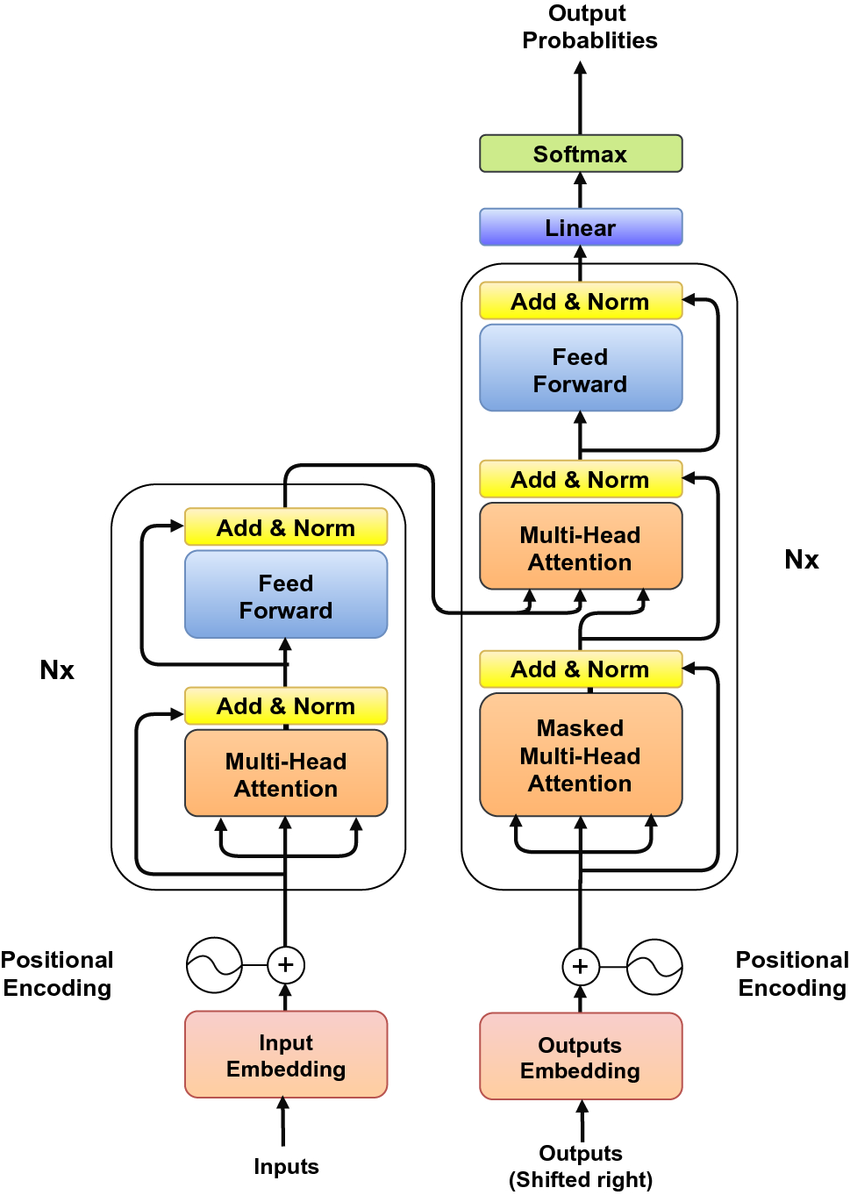
\includegraphics[width=0.65\textwidth]{Transformer-model-architecture.png}
	\caption{معماری ترانسفورمرها}
	\label{fig:transformer_architecture}
\end{figure}

\subsection{جاسازی}
در زبان طبیعی، کلمات به شکل رشته‌های متنی هستند مانند کتاب، ماشین و ... کامپیوترها نمی‌توانند به‌طور مستقیم این کلمات را به شکل رشته‌های متنی پردازش کنند. به همین دلیل، در یادگیری ماشین این کلمات را به شکل یک بردار نمایش می‌دهیم. این بردار بیانگر آن کلمه در مدل است تا ماشین بتواند آن کلمه را پردازش کند.

این بردارها ویژگی‌های کلمه را در فضای عددی نمایش می‌دهند. روش‌های مختلفی برای تبدیل متن به بردار وجود دارند. از جمله این روش‌ها می‌توان به روش‌های \lr{Word2Vec} \cite{mikolov2013distributed} و \lr{GloVe} \cite{pennington2014glove} اشاره کرد.

همان‌طور که در \autoref{fig:word_embedding} نشان داده شده است، هر کلمه که به صورت توکن است، ابتدا در دیکشنری تعریف‌شده پیدا می‌شود و پس از پیدا شدن در دیکشنری، با استفاده از روش‌های تعبیه کردن\footnote{\lr{Embedding}}، هر کلمه به برداری از اعداد تبدیل می‌شود. این جاسازی‌ها شباهت‌های معنایی بین کلمات را مدل‌سازی می‌کنند و کلماتی که از نظر معنایی شبیه به هم هستند، بردار آن‌ها نیز به یکدیگر نزدیک‌تر است. به این ترتیب، کلمات برای مدل‌ها و شبکه‌های عصبی قابل‌فهم می‌شوند \cite{mikolov2013distributed,pennington2014glove}.





 \begin{figure}[h]
 	\centering
 	\begin{minipage}[b]{0.7\textwidth}
 		\centering
 		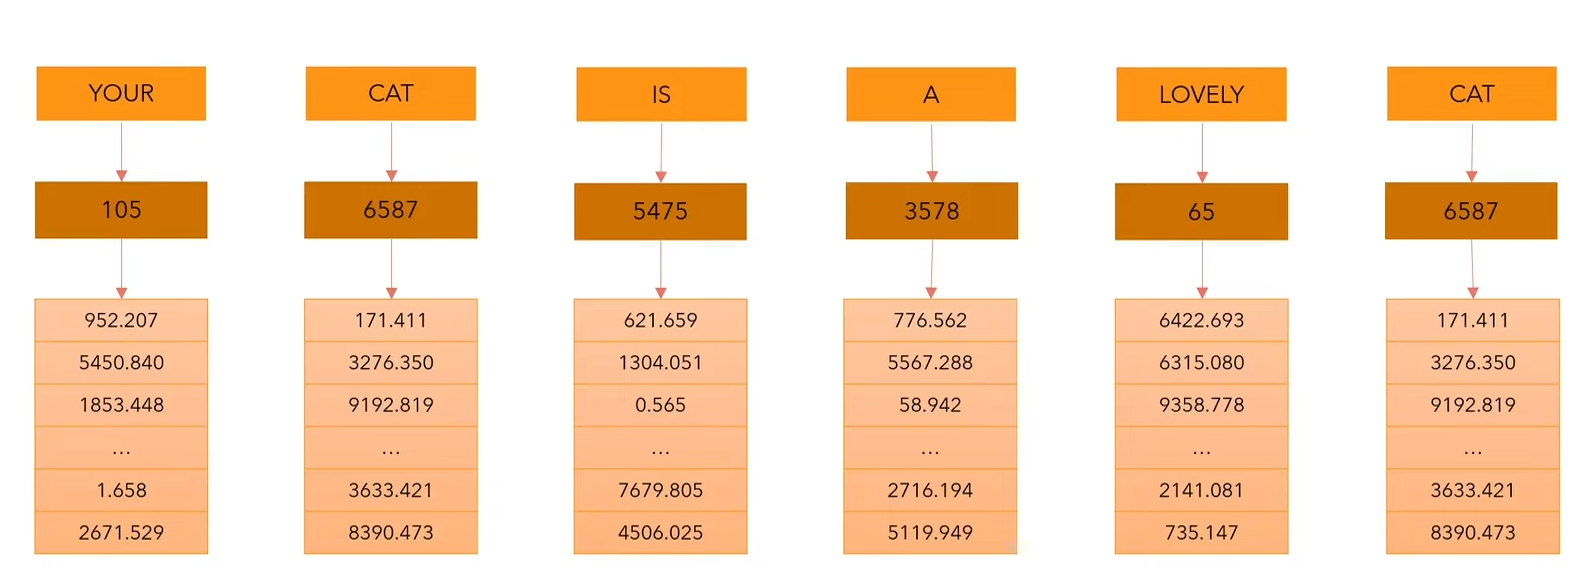
\includegraphics[width=\textwidth]{transformer_images/word_embedding.png}
 		\caption{\lr{جاسازی کلمه ای}}
 		\label{fig:word_embedding}
 	\end{minipage}
 	\hfill
 \end{figure}



\subsection{جاسازی موقعیتی}

هر کلمه را به برداری از اعداد که برای مدل قابل فهم باشد، تبدیل کرده‌ایم. اما مدل‌های ترانسفورمر نمی‌توانند جایگاه هر کلمه را تشخیص دهند. در مدل‌های ترانسفورمر، برخلاف مدل‌های بازگشتی، به دلیل اینکه کلمات به‌صورت موازی وارد می‌شوند، نیاز داریم تا جایگاه هر کلمه را بدانیم. به‌طور مثال، در جملهٔ «من تو را دوست دارم» باید به‌طور دقیق بدانیم که «من» کلمهٔ اول جمله است، «تو» کلمهٔ دوم جمله است و ... .

حال باید به مدل توالی این کلمات را بفهمانیم. بنابراین، نیاز داریم به مدل یک سری اطلاعات اضافی بدهیم به‌طوری‌که مدل توالی کلمات را یاد بگیرد. روش‌های مختلفی برای اضافه‌کردن جاسازی موقعیتی \footnote{\lr{Positional Embedding}} به مدل وجود دارد. در ترانسفورمرها از روش جاسازی موقعیت سینوسی
 \footnote{\lr{Sinusoidal Positional Embedding}} استفاده می‌شود \cite{vaswani2017attention}.



این روش قابل یادگیری نیست و صرفاً از یک سری فرمول‌های ساده برای جاسازی موقعیتی استفاده می‌کند.  
برای موقعیت مشخص \footnote{\lr{pos}} در توالی و بُعد \( i \) در فضای برداری، تعبیه موقعیتی به‌صورت زیر تعریف می‌شود.  

و برای مقادیر زوج:  

\begin{equation}
	PE(pos, 2i) = \sin\left( \frac{pos}{10000^{\frac{2i}{d}}} \right)
	\label{eq:pe_even}
\end{equation}

و برای مقادیر فرد:  

\begin{equation}
	PE(pos, 2i+1) = \cos\left( \frac{pos}{10000^{\frac{2i}{d}}} \right)
	\label{eq:pe_odd}
\end{equation}
	



\begin{itemize}
	\item \( pos \): موقعیت کلمه در توالی است (مثلاً از \( 0 \) تا \( N-1 \) برای یک توالی \( N \)-تایی).
	\item \( i \): شاخص بعد در بردار موقعیتی (از \( 0 \) تا \( d-1 \) برای بعد فضای برداری \( d \)).
	\item \( d \): ابعاد فضای برداری مدل که نشان می‌دهد هر کلمه در چند بعد نمایش داده می‌شود.
	\item \( 10000 \): یک مقدار ثابت برای تنظیم مقیاس توابع تناوبی و ایجاد فرکانس‌های مختلف در ابعاد گوناگون.
\end{itemize}  

همان‌طور که در شکل \autoref{fig:word_embedding_positional_embedding} مشاهده می‌کنید، بعد از جاسازی کلمات، به آن جا سازی موقعیتی اضافه می‌شود. در این روش از توابع سینوس و کسینوس استفاده می‌شود. این توابع موقعیت‌ها را در فضای برداری به‌گونه‌ای نگاشت می‌کنند که مدل بتواند از ترتیب کلمات در توالی آگاه باشد \cite{vaswani2017attention}. این ویژگی به مدل کمک می‌کند تا توالی زمانی را درک کرده و الگوهای زمانی را شبیه‌سازی کند. از مزایای این روش می‌توان به عدم نیاز به آموزش و توزیع متوازن جایگاه کلمات اشاره کرد.

\begin{figure}[h]
	\centering
	\begin{minipage}[b]{0.7\textwidth}
		\centering
		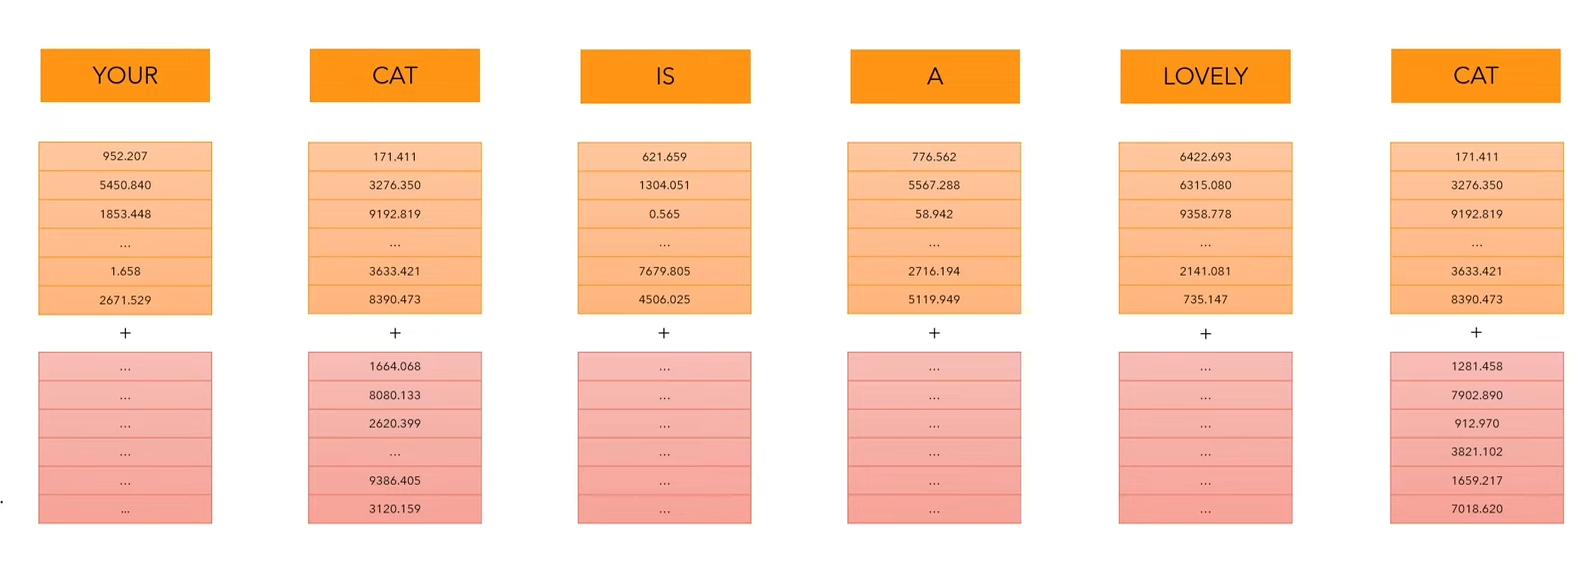
\includegraphics[width=\textwidth]{transformer_images/positional_embedding.png}
		\caption{\lr{جاسازی موقعیتی}}
		\label{fig:word_embedding_positional_embedding}
	\end{minipage}
	\hfill
\end{figure}






\subsection{توجه}



در روش‌ شبکه های بازگشتی، توالی ورودی (مثلاً یک جمله) معمولاً به‌صورت گام‌به‌گام پردازش می‌شد \cite{elman1990finding,hochreiter1997long}. اما در ترانسفورمر می‌خواهیم مدلی داشته باشیم که به هر موقعیت (مثلاً یک کلمه) در توالی نگاه کند و به همهٔ موقعیت‌های دیگر نیز به‌صورت موازی دسترسی داشته باشد. به این مفهوم توجه\footnote{\lr{attention}} می‌گوییم.

به زبان ساده، وقتی توکن (کلمه) \( i \) به توکن‌های دیگر نگاه می‌کند، می‌خواهد بداند کدام توکن‌ها برای تفسیر معنای خودش مهم‌ترند.

به طور مثال در جمله‌ی «یک گربه روی زمین نشسته است» می‌خواهد بداند کلمه‌ی «گربه» به واژه‌ی «نشستن» بیشتر توجه کند یا به «زمین». در این‌جا فعل «نشستن» ارتباط نزدیک‌تری به «گربه» دارد و از نظر معنایی مرتبط‌تر است.


سه تا از اجزای اصلی یک توجه شامل موارد زیر است.

\[
Q = \text{Query (پرسش)}, \quad K = \text{Key (کلید)}, \quad V = \text{Value (مقدار / ارزش)}
\]





در  ضرب شباهت های توجه \footnote{\lr{Scaled Dot-Product Attention}}    \cite{vaswani2017attention}، ابتدا شباهت یا ارتباط بین پرسش \footnote{\lr{Query}} و کلید \footnote{\lr{Key}} را با محاسبهٔ ضرب داخلی \footnote{\lr{Dot Product}} به‌دست می‌آوریم، سپس آن را نرمال می‌کنیم (با تقسیم بر \( d_k \)) و از تابع سافت مکس \footnote{\lr{softmax}} استفاده می‌کنیم تا ضرایب توجه \footnote{\lr{Attention Weights}} را به‌دست آوریم. در نهایت با همین ضرایب، ترکیبی خطی از بردارهای مقدار \footnote{\lr{value}} را می‌گیریم.

فرمول به‌شکل زیر است:

\begin{equation}
	\text{Attention}(Q, K, V) = \text{softmax}\left( \frac{QK^T}{\sqrt{d_k}} \right) V
	\label{eq:attention}
\end{equation}

که در آن:

\[
Q \in \mathbb{R}^{n \times d_k} \quad \text{ماتریس پرسش برای }
\]
\[
K \in \mathbb{R}^{n \times d_k} \quad \text{ماتریس کلید برای }
\]
\[
V \in \mathbb{R}^{n \times d_v} \quad \text{ماتریس مقدار  }
\]



	 \( W^Q, W^K, W^V \in \mathbb{R}^{d_{model} \times d_k} \) ماتریس‌های وزنی قابل آموزش هستند که طی فرآیند یادگیری به‌روزرسانی می‌شوند.
	 
\begin{figure}[h]
	\centering
	\begin{minipage}[b]{0.7\textwidth}
		\centering
		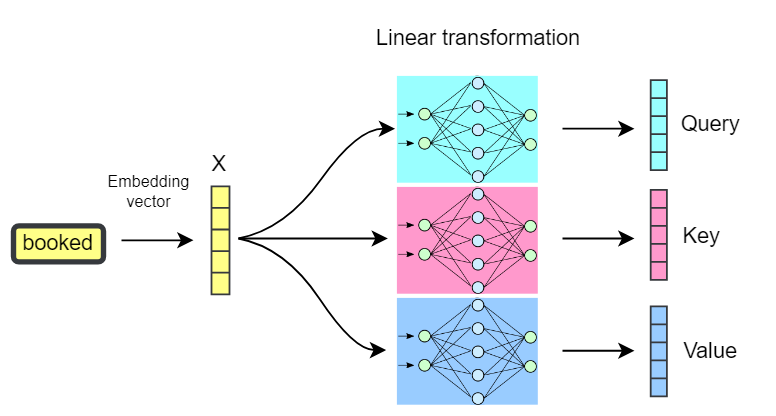
\includegraphics[width=\textwidth]{transformer_images/qkv.png}
		\caption{\lr{نحوه به دست آوردن پرسش، کلید و مقدار}}
		\label{fig:qkv}
	\end{minipage}
	\hfill
\end{figure}


در واقع پرسش، کلید و مقدار با استفاه از mlp  تولید میشود.



تقسیم بر \( d_k \) باعث می‌شود مقدار ضرب داخلی در ابعاد بالا خیلی بزرگ نشود و شیب‌ها گرادیان پایدار بمانند.

\begin{equation}
	\alpha = \text{softmax}\left( \frac{QK^T}{\sqrt{d_k}} \right)
	\label{eq:alpha}
\end{equation}
\(\alpha\) یک ماتریس با ابعاد \( n \times n \) است که سطر \( i \)-ام آن ضرایب توجه برای توکن \( i \) را نشان می‌دهد.

تفسیر ضرایب توجه: هر سطر از \( \alpha \) نشان می‌دهد که توکن فعلی به چه توکن‌هایی در جمله، با چه شدتی توجه می‌کند.



\begin{figure}[h]
	\centering
	\begin{minipage}[b]{0.6\textwidth}
		\centering
		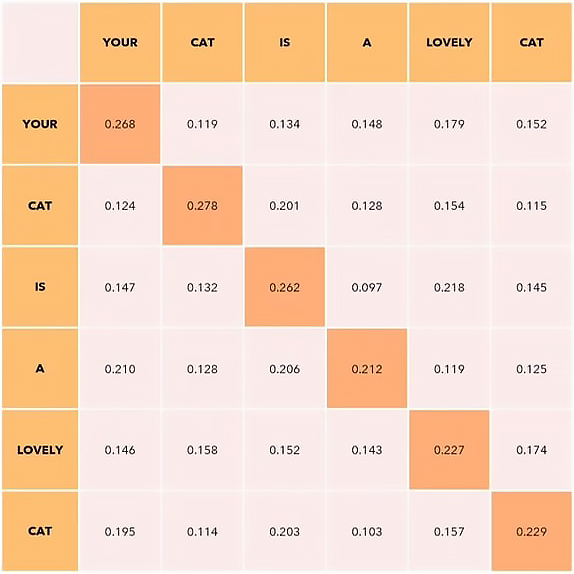
\includegraphics[width=\textwidth]{transformer_images/multi_head_attention_new.png}
		\caption{توجه}
		\label{fig:attention}
	\end{minipage}
	\hfill
	
\end{figure}




\subsection{توجه چند سر}



در ایده چند سری \footnote{\lr{multi head attention}}  
به‌جای آنکه فقط یک‌بار \( Q, K, V \) بسازیم و عملیات توجه را انجام دهیم، چندین مجموعهٔ متفاوت \( Q_i, K_i, V_i \) می‌سازیم (هر کدام یک «سر» \footnote{\lr{head}} نام دارد) و به‌صورت موازی محاسبات توجه را انجام می‌دهیم. سپس خروجی همهٔ این سرها را کنار هم قرار داده \footnote{\lr{concatenate}} و در نهایت با یک ماتریس وزن دیگر ضرب می‌کنیم تا به بعد اصلی بازگردیم.

فرمول مربوط به این ایده به‌شکل زیر است:


\begin{equation}
	\text{head}_i = \text{Attention}(Q_i, K_i, V_i)
	\label{eq:head_i}
\end{equation}


\begin{equation}
	\text{MultiHead}(Q, K, V) = [\text{head}_1 \oplus \cdots \oplus \text{head}_h] W_O
	\label{eq:multihead}
\end{equation}

که در آن \( \oplus \) نشان‌دهندهٔ عمل الحاق \footnote{\lr{concatenate}} است.

ماتریس وزن \( W_O \) به‌شکل زیر است:

\[
W_O \in \mathbb{R}^{(h \cdot d_v) \times d_{\text{model}}}
\]

که \( W_O \) ماتریسی است که خروجی الحاق‌شده را به بعد \( d_{\text{model}} \) برمی‌گرداند.





\begin{figure}[h]
	\centering
	\begin{minipage}[b]{0.9\textwidth}
		\centering
		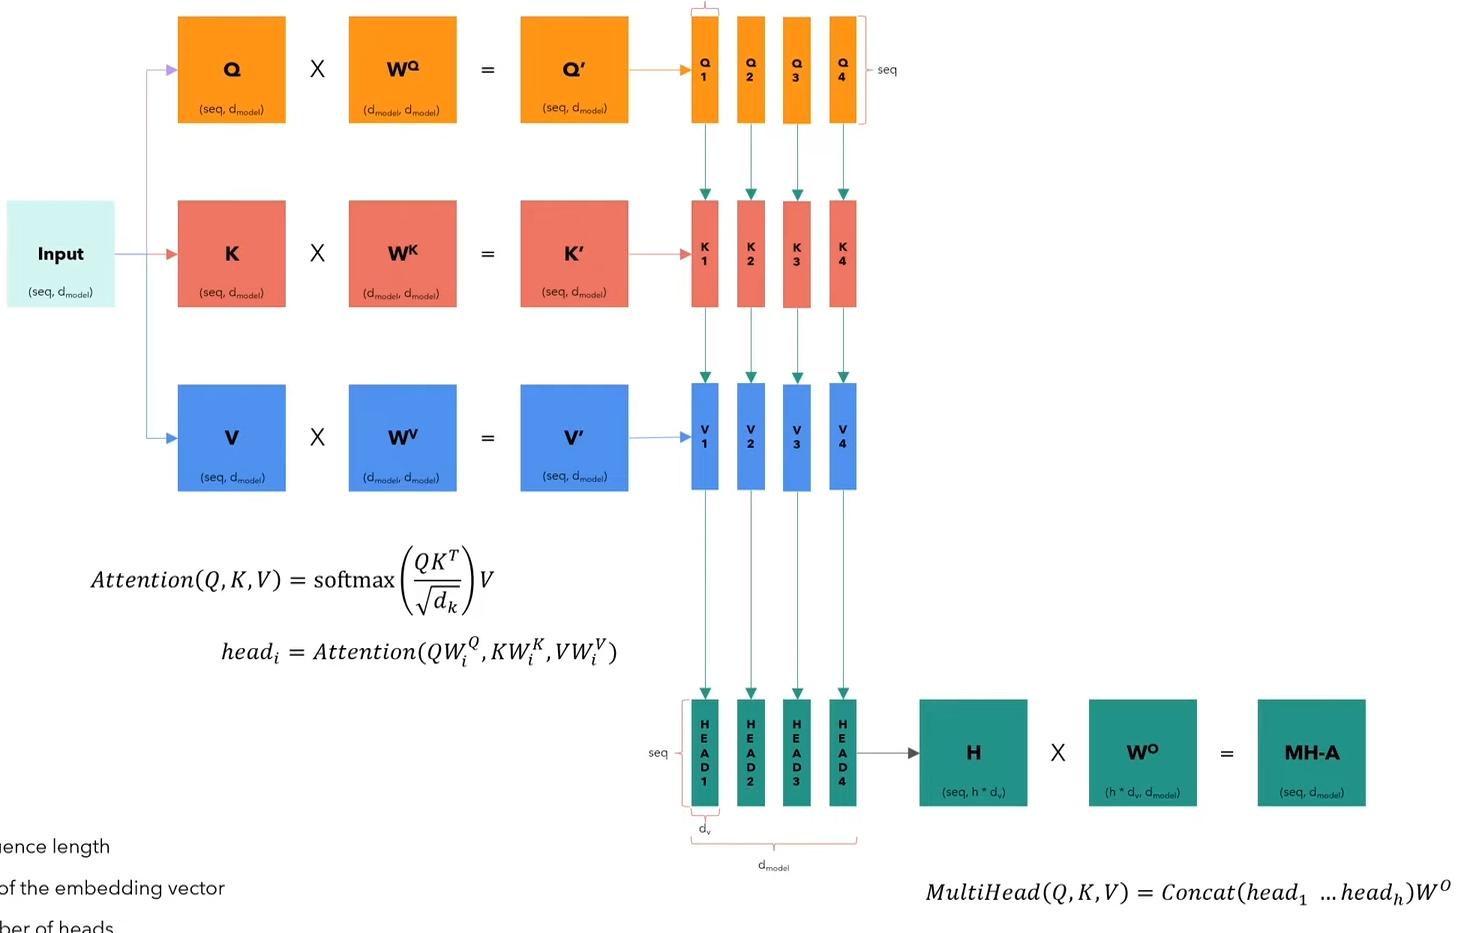
\includegraphics[width=\textwidth]{transformer_images/multi_head_attention.png}
		\caption{توجه چند سر}
		\label{fig:attention}
	\end{minipage}
	\hfill
	
\end{figure}



\subsection*{چرا چندین سر؟}

\textbf{مشاهدهٔ چند منظر متفاوت:} هر  سر می‌تواند الگوهای گوناگونی از وابستگی‌ها را بیاموزد (مثلاً یک سر می‌تواند یاد بگیرد کلمهٔ فعلی با کلمات همسایهٔ نزدیک خود بیشتر مرتبط شود، یک سر  دیگر روی ارتباط با کلماتی در فاصلهٔ دورتری متمرکز باشد، سر دیگر روی مطابقت جنس و تعداد در دستور زبان و ...).

\textbf{افزایش ظرفیت مدل:} با داشتن چند سر ، مدل می‌تواند قدرت بیان بیشتری داشته باشد.

\textbf{ابعاد کمتر در هر سر:} در عمل، اگر \( d_{\text{model}} \) مثلاً 512 باشد، و تعداد سر ها \( h = 8 \)، آنگاه هر سر  ابعادی در حدود \( d_k = 64 \) خواهد داشت؛ و این محاسبات ضرب داخلی را نیز مقیاس‌ پذیر و قابل موازی‌سازی می‌کند.


\subsection{اتصال باقی مانده}
در معماری‌های عمیق، هنگامی که تعداد لایه‌ها زیاد می‌شود، اغلب دچار ناپایداری گرادیان می‌شوند و این مشکل باعث دشواری در آموزش مدل می‌گردد \cite{hochreiter1997long,bengio1994learning}. 

در مبدل ها \cite{vaswani2017attention}، به جای این که خروجی توجه را به‌صورت مستقیم به لایهٔ بعدی بدهیم، ورودی آن را نیز حفظ کرده و به خروجی اضافه می‌کنیم. ایدهٔ اصلی این روش از اتصالات باقی‌مانده \footnote{\lr{Residual Connection}} در شبکه‌های عمیق الهام گرفته شده است \cite{he2016deep}.

اگر \( x \) ورودی به زیرماژول و \( \text{SubLayer}(x) \) خروجی آن زیرماژول باشد، در انتهای کار عبارت زیر را محاسبه می‌کنیم:

\begin{equation}
	x + \text{SubLayer}(x)
	\label{eq:sublayer}
\end{equation}

این جمع به‌صورت عنصر به‌عنصر \footnote{\lr{Element-wise Addition}} انجام می‌شود.


اتصال باقیمانده در مبدل ها چندین مزیت دارد که عبارت اند از:

\subsection*{کمک به جریان یافتن گرادیان}
وقتی ورودی مستقیماً به خروجی اضافه می‌شود، مسیری مستقیم برای عبور شیب (گرادیان) به عقب ایجاد می‌گردد.
در صورت نبود این اتصال، اگر شبکه عمیق شود، گرادیان‌ها ممکن است در لایه‌های پایین محو شوند و عملاً ناپدید شدن گرادیان \footnote{\lr{gradient vanishing}} رخ دهد \cite{hochreiter1997long,bengio1994learning}.

\subsection*{حفظ اطلاعات اصلی (هویت ورودی)}
حتی اگر زیرماژول تغییری در اطلاعات ورودی ایجاد کند، با وجود اتصال باقیمانده \footnote{\lr{Residual Connection}}، ورودی اصلی همواره در خروجی نهایی حضور دارد.
این ویژگی باعث می‌شود در صورت ناکافی‌بودن یادگیری زیرماژول یا در مراحل اولیهٔ آموزش، دست‌کم بخشی از سیگنال (اطلاعات) خام به لایه‌های بالاتر برسد \cite{he2016deep,vaswani2017attention}.

\subsection*{کاهش ریسک تخریب ویژگی‌ها}
در شبکه‌های عمیق، یکی از مشکلات این است که هر لایه ممکن است بخشی از اطلاعات مفید را تخریب کند. اتصال باقی مانده تضمین می‌کند که اگر لایه‌ای به هر دلیل نتوانست الگوی بهینه را یاد بگیرد، اطلاعات قبلی حداقل به‌صورت دست‌نخورده تا حدی منتقل می‌شود.


\section{نرمال سازی لایه ها}

در یادگیری عمیق، نرمال‌سازی \footnote{\lr{Normalization}} داده‌های یک لایه یا فعال‌سازی‌ها، اغلب به سرعت بخشیدن به همگرایی و پایدار کردن آموزش کمک شایانی می‌کند. شاید معروف‌ترین نوع نرمال‌سازی، نرمال سازی بچ \footnote{\lr{Batch Normalization}} باشد که پیش‌تر در کارهای بینایی کانولوشنی\footnote{\lr{CNN}} بسیار مورداستفاده قرار گرفت \cite{ioffe2015batch}.

نرمال سازی لایه ها \footnote{\lr{Layer Normalization}} روشی جایگزین است که در ترانسفورمر استفاده می‌شود \cite{ba2016layer,vaswani2017attention}. علت اصلی این انتخاب، ماهیت توالی‌محور \footnote{\lr{sequence}} بودن داده‌ها در پردازش زبان طبیعی و عدم تمایل به وابستگی به آمار مینی‌بچ \footnote{\lr{mini-batch}} است.


\subsection*{نرمال سازی بچ}
در نرمال سازی بچ ها، برای نرمال‌سازی، میانگین و واریانس روی تمام نمونه‌های موجود در مینی‌بچ (و نیز در طول ابعاد ویژگی) محاسبه می‌شود \cite{ioffe2015batch}.
این موضوع در پردازش زبان طبیعی کمی دردسرساز است؛ چون ترتیب توکن‌ها، طول جمله‌ها و حتی اندازهٔ مینی‌بچ ممکن است نامنظم باشد.
همچنین به خاطر تنوع طول توالی‌ها، پیاده‌سازی نرمال سازی بچ ها می‌تواند پیچیده شود.

\subsection*{نرمال سازی لایه ها}
در  نرمال سازی لایه ها، برای هر توکن به‌صورت جداگانه (در طول بُعد ویژگی)، میانگین \footnote{\lr{mean}} و واریانس \footnote{\lr{variance}} گرفته می‌شود \cite{ba2016layer}.
فرض کنید در یک لایه، بردار \( h_i \in \mathbb{R}^{d_{\text{model}}} \) مربوط به توکن \( i \) باشد؛ یعنی ابعاد ویژگی آن \( d_{\text{model}} \) است. ما میانگین \( \mu_i \) و واریانس \( \sigma_i^2 \) را از اجزای این بردار محاسبه می‌کنیم:

\begin{equation}
	\mu_i = \frac{1}{d_{\text{model}}} \sum_{k=1}^{d_{\text{model}}} h_{i,k}, \quad
	\sigma_i^2 = \frac{1}{d_{\text{model}}} \sum_{k=1}^{d_{\text{model}}} (h_{i,k} - \mu_i)^2
	\label{eq:mean_variance}
\end{equation}


سپس نرمال‌سازی برای هر مؤلفهٔ \( k \) در بردار توکن \( i \) به شکل زیر انجام می‌شود:

\begin{equation}
	\hat{h}_{i,k} = \frac{h_{i,k} - \mu_i}{\sqrt{\sigma_i^2 + \epsilon}}
	\label{eq:normalized_h}
\end{equation}

در نهایت، برای این‌که مدل بتواند مقیاس و بایاس جدیدی یاد بگیرد، شبیه بچ نرم ، دو پارامتر \( \gamma \) و \( \beta \) نیز در طول بعد ویژگی اعمال می‌شوند:

\begin{equation}
	\text{LayerNorm}(h_i) = \gamma \odot \hat{h}_i + \beta
	\label{eq:layernorm}
\end{equation}


که در آن \( \gamma, \beta \in \mathbb{R}^{d_{\text{model}}} \) هستند و \( \odot \) ضربِ عنصر به عنصر است \cite{ba2016layer}.

\subsection*{مزایای نرمال سازی لایه در مبدل ها}

\begin{itemize}
	\item \textbf{بی‌نیازی از وابستگی به ابعاد مینی‌بچ:}  
	با نرمال سازی لایه، می‌توان حتی با اندازهٔ مینی‌بچ برابر ۱ نیز به‌خوبی آموزش دید، چراکه آمارها وابسته به ابعاد ویژگی‌اند و نه مینی‌بچ \cite{ba2016layer}.
	
	\item \textbf{پایدارسازی توزیع فعال‌سازی‌ها:}  
	زمانی که مدل در حال یادگیری است، توزیع‌های داخلی لایه‌های میانی ممکن است تغییر کند.\footnote{\lr{Internal Covariate Shift}} نرمال سازی لایه با نرمال‌سازی این توزیع، آموزش را پایدارتر و سریع‌تر می‌کند \cite{ioffe2015batch,ba2016layer}.
	
	\item \textbf{سازگاری با داده‌های توالی‌محور:}  
	هر توکن را جداگانه نرمال می‌کند و نگرانی‌ای بابت ترتیب طول جمله‌ها، یا قرار گرفتن چند جملهٔ کوتاه/بلند در یک مینی‌بچ نداریم \cite{vaswani2017attention}.
\end{itemize}

در معماری مبدل ها، پس از خروجی هر زیرماژول، مراحل به‌شکل زیر است:

\subsection{اتصال باقی مانده}
ابتدا ورودی همان زیرماژول (مثلاً بردار \( x \)) را با خروجی زیرماژول (\( \text{SubLayer}(x) \)) جمع می‌کنیم. حاصل این جمع را می‌توان چنین نوشت:


\begin{equation}
	z = x + \text{SubLayer}(x)
\end{equation}


این \( z \) حالا ترکیبی از اطلاعات اصلی ورودی و اطلاعات یادگرفته‌شده توسط \lr{SubLayer} است.

\paragraph{نرمال سازی لایه}
سپس این بردار \( z \) را وارد لایهٔ \lr{LayerNorm} می‌کنیم.

\[
y = \text{LayerNorm}(z)
\]

خروجی نهایی را می‌توان به لایهٔ بعدی پاس داد یا به مرحلهٔ بعدی در همین لایه.

به‌عبارتی اگر بخواهیم در یک فرمول واحد بیان کنیم:

\[
\text{Add \& Norm} = \text{LayerNorm}\bigl(x + \text{SubLayer}(x)\bigr)
\]


\section{رمزگشا}
رمزگشا در معماری ترانسفورمرها وظیفهٔ تولید خروجی نهایی را بر عهده دارد. این خروجی معمولاً می‌تواند توالی هدف \footnote{\lr{Target Sequence}} باشد، مانند ترجمه یک جمله یا پیش‌بینی توکن‌های بعدی در یک توالی \cite{vaswani2017attention}. 

در این بخش، رمزگشا دو ورودی اصلی دارد:  
1. توالی هدف که معمولاً به‌صورت خودکار تولید می‌شود (مثلاً در ترجمهٔ ماشینی یا تولید متن)،  
2. نمایش اطلاعات کدشده که توسط انکودر تولید شده است و شامل ویژگی‌های استخراج‌شده از توالی ورودی می‌باشد.  

رمزگشا از این ورودی‌ها استفاده می‌کند تا به‌صورت گام‌به‌گام، خروجی نهایی خود را تولید کند \cite{bahdanau2014neural,sutskever2014sequence}.

همان‌طور که در شکل \ref{fig:Decoder} مشاهده می‌کنید،  رمز گشا دو ورودی دارد.

\begin{figure}[h]
	\centering
	\begin{minipage}[b]{0.25\textwidth}
		\centering
		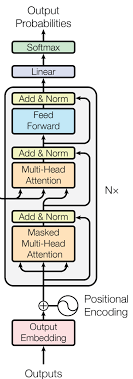
\includegraphics[width=\textwidth]{transformer_images/decoder.png}
		\caption{}
		\label{fig:Decoder}
	\end{minipage}
	\hfill
\end{figure}

تمامی بخش‌های رمزگشا مانند رمزگدار هستند اما در دیکودر توجه چند سر ماسک شده \footnote{\lr{Masked Multi-Head Attention}} وجود دارد \cite{vaswani2017attention}.



\section{توجه  چند سری ماسک شده}
در مبدل‌ها، مکانیزم توجه چند سری \footnote{\lr{Multi-Head Attention}} در بخش دیکودر به‌صورت ماسک شده \footnote{\lr{Masked}} پیاده‌سازی می‌شود تا مدل نتواند توکن‌های آینده را ببیند و به‌صورت خودبازگشتی \footnote{\lr{Autoregressive}} توکن بعدی را پیش‌بینی کند \cite{vaswani2017attention}.


در واقع ایده اصلی استفاده از ماسک جلوگیری از مشاهده آینده است.

در معماری‌های خودبازگشتی، مدل در گام \( i \) از دیکودر تنها باید به توکن‌های قبلی \( \{ y_1, \dots, y_{i-1} \} \) دسترسی داشته باشد؛ اما نه به توکن‌های \( \{ y_{i+1}, y_{i+2}, \dots \} \). اگر مدل بتواند توکن‌های آینده را «نگاه» کند، پیش‌بینی توکن بعدی آسان و غیرواقعی می‌شود (مشکل نشت اطلاعات) \cite{bahdanau2014neural,sutskever2014sequence}.

به همین دلیل در توجه چند سری ماسک شده در  دیکودر، از یک ماتریس ماسک \( M \) استفاده می‌کنیم که اجازه نمی‌دهد هر توکن به توکن‌های آینده‌اش توجه کند.

\section{مثال عددی توجه ماسک شده}
فرض کنید دنبالهٔ 4 توکنی داریم:
\[
[y_1, y_2, y_3, y_4]
\]
خروجی ضرب داخلی  (قبل از \texttt{softmax}) یک ماتریس \(4 \times 4\) خواهد بود:
\[
S =
\begin{bmatrix}
	s_{1,1} & s_{1,2} & s_{1,3} & s_{1,4} \\
	s_{2,1} & s_{2,2} & s_{2,3} & s_{2,4} \\
	s_{3,1} & s_{3,2} & s_{3,3} & s_{3,4} \\
	s_{4,1} & s_{4,2} & s_{4,3} & s_{4,4}
\end{bmatrix}
\]

\begin{itemize}
	\item \textbf{سطر 1 (توکن اول)}: تنها می‌تواند خودش (\textbf{ستون 1}) را ببیند، اما \textbf{ستون‌های 2 تا 4} ماسک می‌شوند.
	\item \textbf{سطر 2 (توکن دوم)}: می‌تواند به \textbf{ستون‌های 1 و 2} نگاه کند، اما \textbf{ستون‌های 3 و 4} ماسک می‌شوند.
	\item \textbf{سطر 3}: می‌تواند \textbf{ستون‌های 1، 2 و 3} را ببیند، اما \textbf{ستون 4} ماسک می‌شود.
	\item \textbf{سطر 4}: می‌تواند به \textbf{ستون‌های 1، 2، 3 و 4} دسترسی داشته باشد (چهارمین توکن می‌تواند توکن‌های قبلی را ببیند. همچنین این توکن \textbf{خودش} نیز معمولاً در دسترس است . بسته به پیاده‌سازی، ممکن است توکن فعلی از خودش نیز استفاده کند یا نه. در معماری استاندارد، سطر \( i \) معمولاً به ستون \( i \) هم دسترسی دارد).
\end{itemize}

در عمل، ماتریس ماسک \( M \) به شکل زیر خواهد بود (با نشانه‌گذاری پایین‌مثلثی):


\[
M =
\begin{bmatrix}
	0 & -\infty & -\infty & -\infty \\
	0 & 0 & -\infty & -\infty \\
	0 & 0 & 0 & -\infty \\
	0 & 0 & 0 & 0
\end{bmatrix}
\]

به این ترتیب، پس از جمع شدن با \( S \) و اجرای \texttt{softmax} در هر سطر، ضرایب توجه ستون‌های ماسک‌شده به صفر میل می‌کنند \cite{vaswani2017attention}.

 
\section{مبدل های بینایی}

ایده ترانسفورمرها در حوزهٔ بینایی \footnote{\lr{vision transformer}} از تعمیم ترانسفورمر متن به تصاویر به وجود آمده است \cite{dosovitskiy2020image}.

ما در این بخش از مبدل های بینایی برای وظیفه کلاس‌بندی استفاده می‌کنیم.

در روش‌های متداول برای پردازش تصویر، از کانولشن \footnote{\lr{convolution}} ‌های متوالی استفاده می‌کردند؛ اما در ترانسفورمرها تصاویر به پچ‌های مختلف شکسته می‌شوند \cite{dosovitskiy2020image}. هر پچِ شکسته‌شده از تصویر می‌تواند با سایر پچ‌ها به‌صورت موازی وارد مکانیزم توجه  شود و شباهت یا ارتباطشان با یکدیگر سنجیده شود. در بخش‌های بعد، به‌طور مفصل روند انجام این کار را توضیح خواهیم داد.


\subsection{جاسازی پچ ها در مبدل های بینایی}
در ترانسفورمرهای مبتنی بر متن، هر کلمه به توکن تبدیل می‌شود و سپس هر کلمه به برداری تبدیل می‌گردد. این بردارها پس از افزودن جاسازی موقعیتی وارد مکانیزم توجه می‌شوند \cite{vaswani2017attention}. 

حال همین ایده در تصویر پیاده‌سازی شده است. همان‌طور که در شکل \ref{fig:image to patch in vision transformer} مشاهده می‌کنید، در مبدل های بینایی، به‌جای استفاده از عملیات کانولوشن‌های متوالی که در شبکه‌های پیچشی \footnote{\lr{convolutional neural network}} مرسوم است \cite{lecun1998gradient,krizhevsky2012imagenet,he2016deep}، تصویر را به بلاک‌های غیرهم‌پوشان (\(P \times P\)) تقسیم می‌کنیم. این کار علاوه بر ساده‌سازی موازی‌سازی، به مدل اجازه می‌دهد از سازوکار توجه برای ارتباط بین این بلاک‌ها استفاده کند \cite{dosovitskiy2020image}.

\begin{figure}[h]
	\centering
	\begin{minipage}[b]{0.9\textwidth}
		\centering
		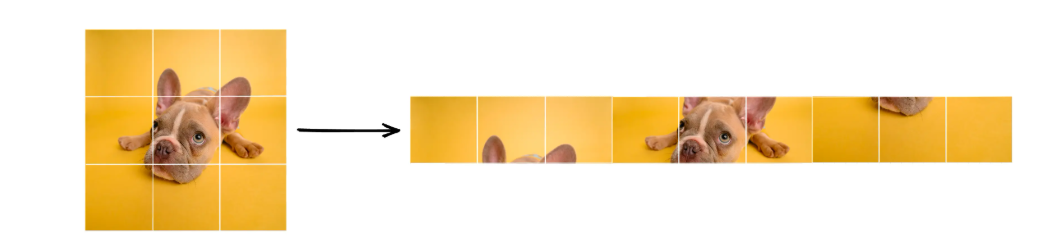
\includegraphics[width=\textwidth]{transformer_images/image_patch_embedding.png}
		\caption{بخش بندی تصاویر}
		\label{fig:image to patch in vision transformer}
	\end{minipage}
	\hfill
\end{figure}

\subsection{شکل پچ‌ها:}
فرض کنید ابعاد تصویر ورودی (\(H \times W \times C\)) باشد. به‌عنوان مثال، اگر اندازهٔ تصویر \(224 \times 224 \times 3\) باشد، طول و عرض تصویر به‌ترتیب \(224\) و تصویر دارای سه کانال رنگی است:

\[
H = 224, \quad W = 224, \quad C = 3
\]


حال اگر اندازهٔ هر پچ (\(P \times P\)) باشد (برای نمونه \(16 \times 16\))، تصویر به‌صورت یک جدول مشبک از پچ‌های کوچک تقسیم می‌شود.  
به هر پچ می‌توان مانند یک «کاشی» از تصویر نگاه کرد:
- پچ اول: مختصات \((0 \text{ تا } 15 \text{ در ارتفاع}) \) و \((0 \text{ تا } 15 \text{ در عرض})\)،  
- پچ دوم: مختصات \((0 \text{ تا } 15 \text{ در ارتفاع}) \) و \((16 \text{ تا } 31 \text{ در عرض})\)،  
- و به همین ترتیب تا کل تصویر پوشش داده شود.



\subsection{تعداد پچ‌ها:}
اگر پچ‌ها بدون هم‌پوشانی باشند، ابعاد پچ باید بر ابعاد تصویر بخش‌پذیر باشد.  

- تعداد پچ‌های افقی: \(\frac{W}{P}\)  
- تعداد پچ‌های عمودی: \(\frac{H}{P}\)  

در مجموع:  
\begin{equation}
	\left(\frac{H}{P}\right) \times \left(\frac{W}{P}\right) = \frac{H}{P} \times \frac{W}{P}.
	\label{eq:grid_size}
\end{equation}


برای مثال اگر:
\[
H = 224, \quad W = 224, \quad P = 16:
\]
\[
\frac{224}{16} = 14 \quad \Rightarrow \quad 14 \times 14 = 196 \quad (\text{تعداد پچ‌ها}).
\]

در اکثر نسخه‌های مبدل‌های بینایی، پچ‌ها بدون هم‌پوشانی \footnote{\lr{Non-overlapping}} هستند. اندازه پچ‌های کوچک باعث می‌شود تعداد پچ‌ها زیاد شود و در نتیجه هزینه توجه بالا رود. از طرفی، پچ‌های بزرگ هزینه توجه را کاهش می‌دهند؛ اما ممکن است جزییات محلی \footnote{\lr{Local Details}} را از دست بدهیم \cite{dosovitskiy2020image}.


\subsection{بردارکردن هر پچ}
هر پچ دارای ابعاد \((P \times P \times C)\) است. برای مثال اگر \(P=16\) و \(C=3\)، آنگاه پچ ابعاد \(16 \times 16 \times 3\) خواهد داشت.  
برای این‌که بتوانیم پچ‌ها را مانند «توکن»‌های پردازش زبان ظبیعی به مبدل ها بدهیم، باید آن‌ها را به یک بردار یک ‌بعدی تبدیل کنیم. در صورت قرار دادن پیکسل‌های پچ به‌صورت ردیفی \footnote{\lr{Row-major}}، طول این بردار خواهد بود:

\begin{equation}
	P \times P \times C = P^2 \times C.
	\label{eq:patch_volume}
\end{equation}

در مثال \((16 \times 16 \times 3)\)، طول بردار می‌شود \(768\).


\section{اعمال لایهٔ خطی}
بعد از کنار هم چیدن پچ ها \footnote{\lr{Flatten}}، معمولاً یک لایهٔ خطی \footnote{\lr{Fully-Connected Layer}} روی این بردار اعمال می‌شود تا آن را به بعد \(d_{\text{model}}\) (مثلاً 768 یا 1024) ببرد. در حقیقت، این لایه یک تبدیل ویژگی \footnote{\lr{Feature Transformation}} انجام می‌دهد تا همه پچ‌ها یک نمایندگی (تعبیه شده) با ابعاد یکنواخت \(d_{\text{model}}\) پیدا کنند:
\[
(P^2 \times C) \quad \rightarrow \quad d_{\text{model}}
\]

\begin{figure}[h]
	\centering
	\begin{minipage}[b]{0.9\textwidth}
		\centering
		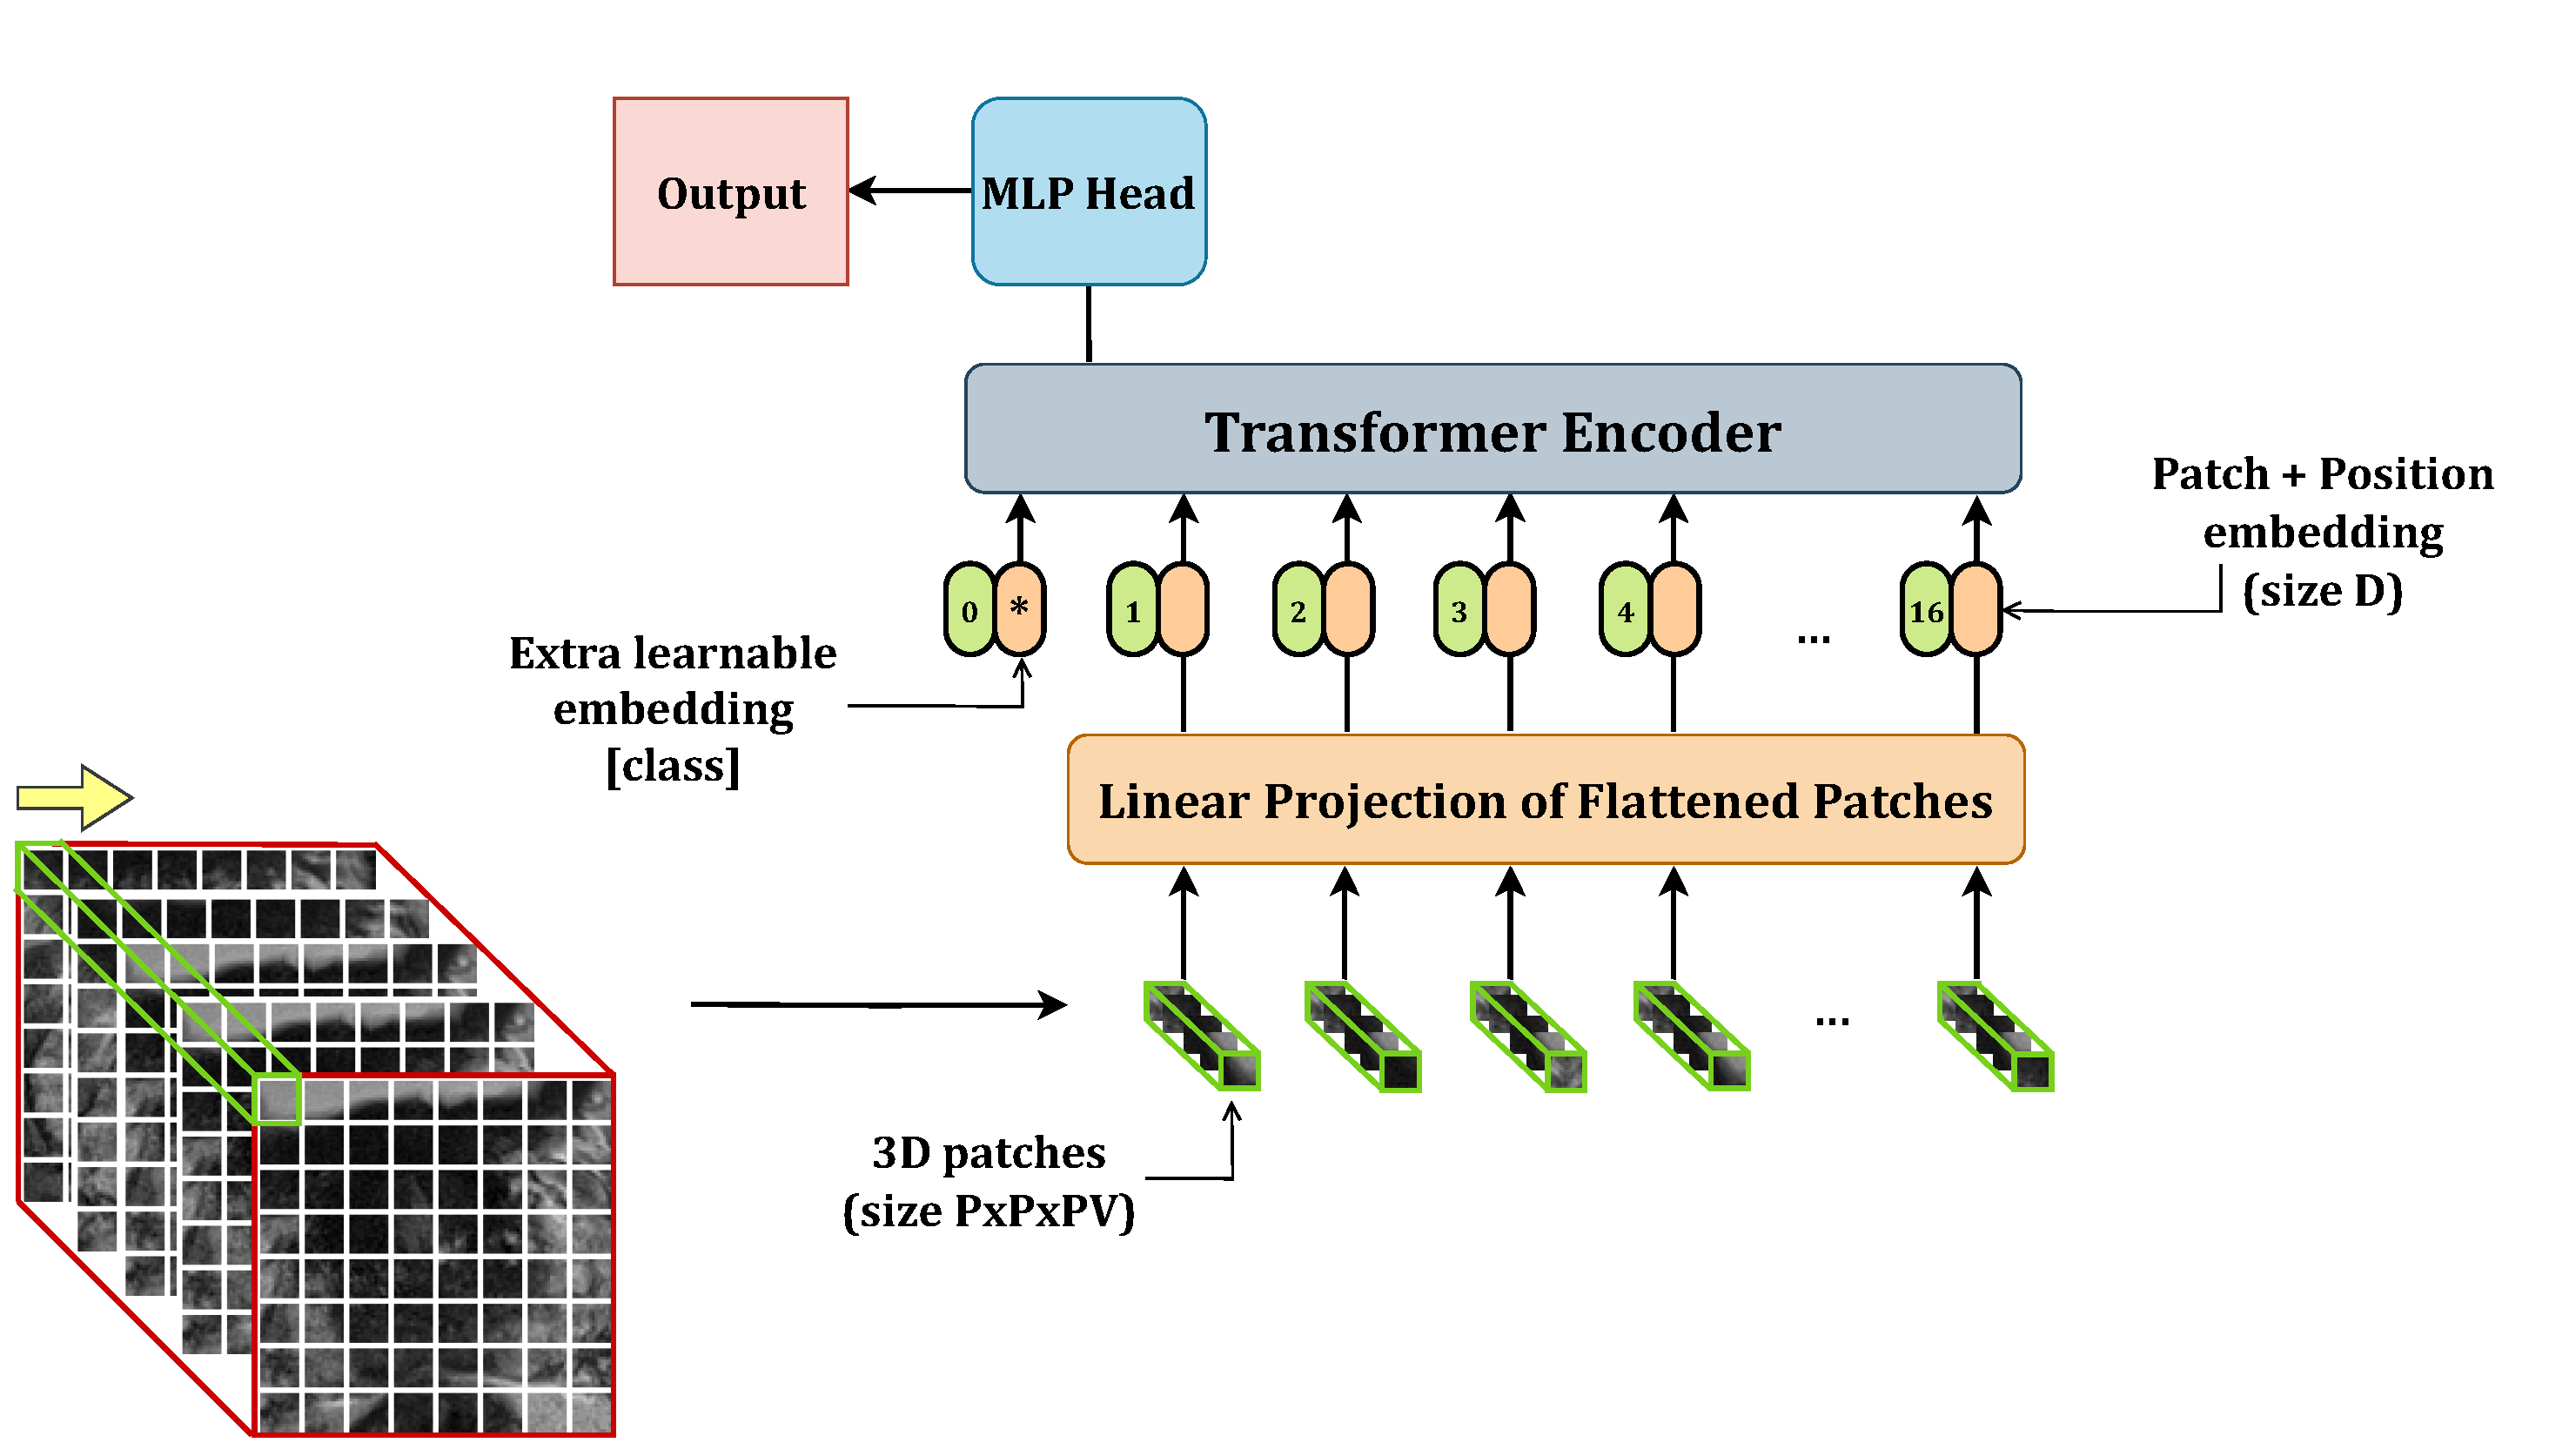
\includegraphics[width=\textwidth]{transformer_images/vision_transformer_embedding.png}
		\caption{مبدل های بینایی}
		\label{fig:Embedding Vision Transformer}
	\end{minipage}
	\hfill
\end{figure}

این مرحله شبیه ساخت توکن در پردازش زبان طبیعی است؛ با این تفاوت که در پردازش زبان طبیعی، توکن «کلمه» یا «زیرکلمه» است و از قبل دارای بردار تعبیه‌شده جاساز شده بوده است \cite{vaswani2017attention}. در مبدل های بینایی \cite{dosovitskiy2020image}، ما ابتدا باید تصاویر را پچ کنیم و سپس بردارهای  جاساز را از این پچ‌ها به دست آوریم.

ترانسفورمر نیاز دارد ورودی‌اش توالی توکن‌ها باشد. در پردازش زبان طبیعی توالی کلمات داریم، در مبدل های بینایی توالی «پچ»‌ها:
\[
\{ x_{\text{patch}_1}, x_{\text{patch}_2}, \dots, x_{\text{patch}_N} \}.
\]
هر پچ اکنون یک بردار \(d_{\text{model}}\)-بعدی است. پس یک مجموعه با طول \(N\) (تعداد پچ‌ها) و عرض \(d_{\text{model}}\) خواهیم داشت.  
اگر عدد پچ‌ها \(N\) باشد (مثلاً 196)، ترانسفورمر می‌تواند با مکانیزم توجه خود سر، وابستگی  میان پچ‌ها را یاد بگیرد: کدام بخش از تصویر برای کدام بخش دیگر مهم‌تر است\cite{vaswani2017attention,dosovitskiy2020image}.

معمولاً پچ‌ها را به‌صورت ردیفی شماره‌گذاری می‌کنند (ابتدا پچ‌های ردیف بالایی از چپ به راست، سپس ردیف بعدی و …)، تا مدل در صورت نیاز بتواند از موقعیت‌ها، اطلاعات مکانی تقریبی داشته باشد.  
در عمل، چون قصد داریم (در مراحل بعد) به هر پچ یک جاسازی موقعیتی هم اضافه کنیم، مکان دقیق هر پچ در بُعد دوم (ویژگی) کد می‌شود.

در مبدل بینایی \cite{dosovitskiy2020image} دیگر به کانولوشن وابسته نیستیم. در عوض، از جاسازی استفاده می‌شود.  
تقسیم  کردن تصویر به بلاک‌های \((P \times P)\)، کنار هم چیدن و تبدیل آن به جاساز همگی عملیات ریاضی ساده‌ای هستند که به‌راحتی روی \lr{GPU}/\lr{TPU} قابل موازی‌سازی‌اند.

\subsection{توکن کلاس بندی}
توکن کلاس بندی \footnote{\lr{Cls Token}} یک بردار ویژه است که به ابتدای دنبالهٔ ورودی اضافه می‌شود و نقش آن، خلاصه‌کردن اطلاعات کل ورودی (چه متن، چه تصویر) است \cite{devlin2018bert,dosovitskiy2020image}.

در مبدل بینایی، این توکن در ابتدای پچ‌های تصویری قرار می‌گیرد.  
این توکن یک بردار با ابعاد \(d_{\text{model}}\) است (همان ابعاد سایر توکن‌ها) و پارامتری یادگرفتنی محسوب می‌شود؛ یعنی مدل طی آموزش، مقادیر آن را برای ذخیره و تجمیع اطلاعات بهینه می‌کند.

در وظایف دسته‌بندی کلاس بندی، هدف این است که یک پیش‌بینی کلی برای کل ورودی (مثلاً یک جمله یا یک تصویر) ارائه دهیم؛ توکن کلاس بندی دقیقاً همین وظیفه را بر عهده دارد \cite{devlin2018bert}. این توکن از طریق مکانیزم توجه چند سر در مبدل ها با تمامی توکن‌های دیگر (پچ‌های تصویر) ارتباط می‌گیرد و اطلاعات مهم آن‌ها را در لایه‌های مختلف مبدل ها را به‌صورت تجمعی یاد می‌گیرد. به عبارتی، توکن کلاس بندی نقش نماینده کل تصویر یا متن را بر عهده دارد.

توکن کلاس بندی از طریق ضرب داخلی در مکانیزم توجه، می‌تواند به تمام پچ‌ها نگاه کند و با ضرایب توجه (\(\alpha\)) مشخص کند که از هر پچ چه مقدار اطلاعات بگیرد. بدین‌ترتیب، به‌طور ضمنی یاد می‌گیرد روی ویژگی‌هایی که برای دسته‌بندی مهم هستند (نظیر الگوها، اشکال و بخش‌های کلیدی تصویر) متمرکز شود.

در طول لایه‌های ترانسفورمر، توکن کلاس بندی نقش محوری در خلاصه‌سازی بازنمایی کل تصویر ایفا می‌کند. این توکن به‌صورت پارامتر قابل یادگیری تعریف شده و در طول فرآیند آموزش به‌روزرسانی می‌شود \cite{devlin2018bert,dosovitskiy2020image}.

\subsection{رمزگذار در مبدل های بینایی}

رمزگذار در ترانسفورمرها همانند مبدل اصلی است \cite{vaswani2017attention}، با این تفاوت که در مبدل های بینایی \cite{dosovitskiy2020image} دیگر به رمزگشا نمی‌رویم. پس از عبور از بلاک‌های ترانسفورمر، در ساده‌ترین حالت یک لایه خطی \footnote{\lr{Fully Connected}} یا یک لایه \lr{MLP} \footnote{\lr{Multi-Layer Perceptron}} بر روی بردار نهایی اعمال می‌شود و این لایه‌ها به تعداد کلاس‌ها خروجی می‌دهند.  
سپس خروجی هر لایه با گذر از تابع سافت مکس \footnote{\lr{softmax}} به احتمال هر کلاس تبدیل می‌شود و در نهایت مدل کلاس با بیشترین احتمال را به‌عنوان خروجی پیش‌بینی می‌کند.

\begin{figure}[h]
	\centering
	\begin{minipage}[b]{0.9\textwidth}
		\centering
		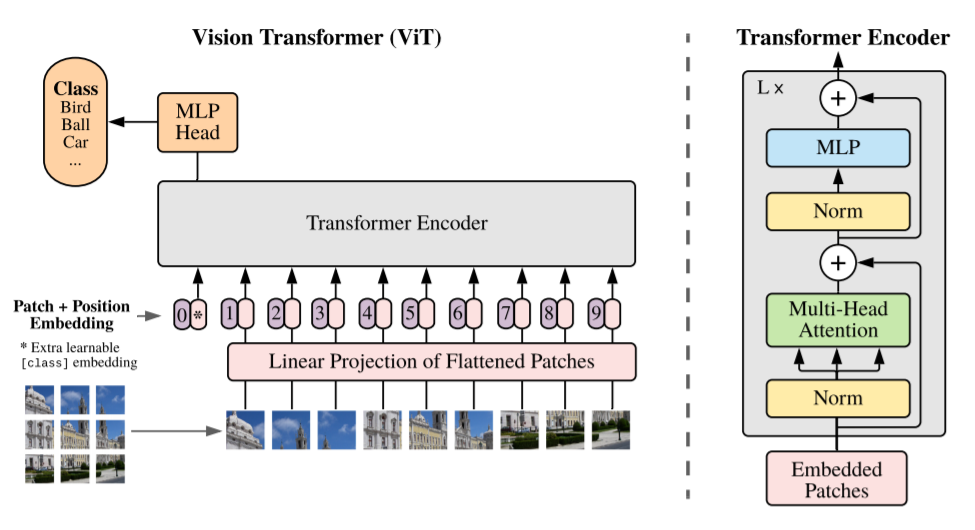
\includegraphics[width=\textwidth]{transformer_images/vision_transformer_after_embedding.png}
		\caption{توکن توجه در مبدل های بینایی}
		\label{fig:Cls Token In Vision Transformer}
	\end{minipage}
	\hfill
\end{figure}

در مبدل ها، هر لایه رمزگشا و رمزگذار با پردازش عمیق‌تر روی توالی ورودی، می‌تواند نمایش بهتری از ویژگی‌ها به‌دست بیاورد \cite{vaswani2017attention}. تکرار چندین‌باره رمزگشا یا رمزگذار موجب می‌شود مدل بتواند ساختارهای پیچیده‌ای را یاد بگیرد و کیفیت و دقت آن در شناسایی توالی‌های طولانی و معانی پنهان افزایش یابد \cite{vaswani2017attention,dosovitskiy2020image}. 
در نتیجه، مدل با تعداد لایه‌های بیشتر اغلب عملکرد بهتری از خود نشان می‌دهد.

   
   
\section{مبدل پنجره‌ای متحرک}
ایده مبدل پنجره‌ای متحرک \footnote{\lr{Swin Transformer}} از ترکیب چند مفهوم کلیدی در مدل‌های ترانسفورمر و شبکه‌های پیچشی شکل گرفت \cite{vaswani2017attention,he2016deep,liu2021swintransformer}.

یکی از بزرگترین مشکلات در ترانسفورمرهای اولیه، نیاز به محاسبات بسیار زیاد در زمانی بود که تصویر ورودی ابعاد بسیار بزرگی داشت \cite{dosovitskiy2020image}. در ترانسفورمر معمولی هر پچ به تمامی پچ‌های دیگر توجه  می‌کرد و در مواقعی که تعداد پچ‌ها زیاد می‌شد، هزینه محاسباتی و حافظه به‌شدت افزایش پیدا می‌کرد.

در شبکه‌های پیچشی، معماری معمولاً به‌صورت سلسله‌مراتبی پیش می‌رود \cite{he2016deep}؛ یعنی ابتدا ویژگی‌های محلی استخراج می‌شود، سپس با عمیق‌تر شدن لایه‌ها، این ویژگی‌ها در سطوح بالاتر با یکدیگر ترکیب می‌شوند. در مبدل پنجره‌ای متحرک \cite{liu2021swintransformer}، با دانش بر این موضوع توانسته‌اند هم هزینه‌های محاسباتی را کاهش دهند و هم دقت مدل را افزایش دهند.

\begin{figure}[h]
	\centering
	\begin{minipage}[b]{1\textwidth}
		\centering
		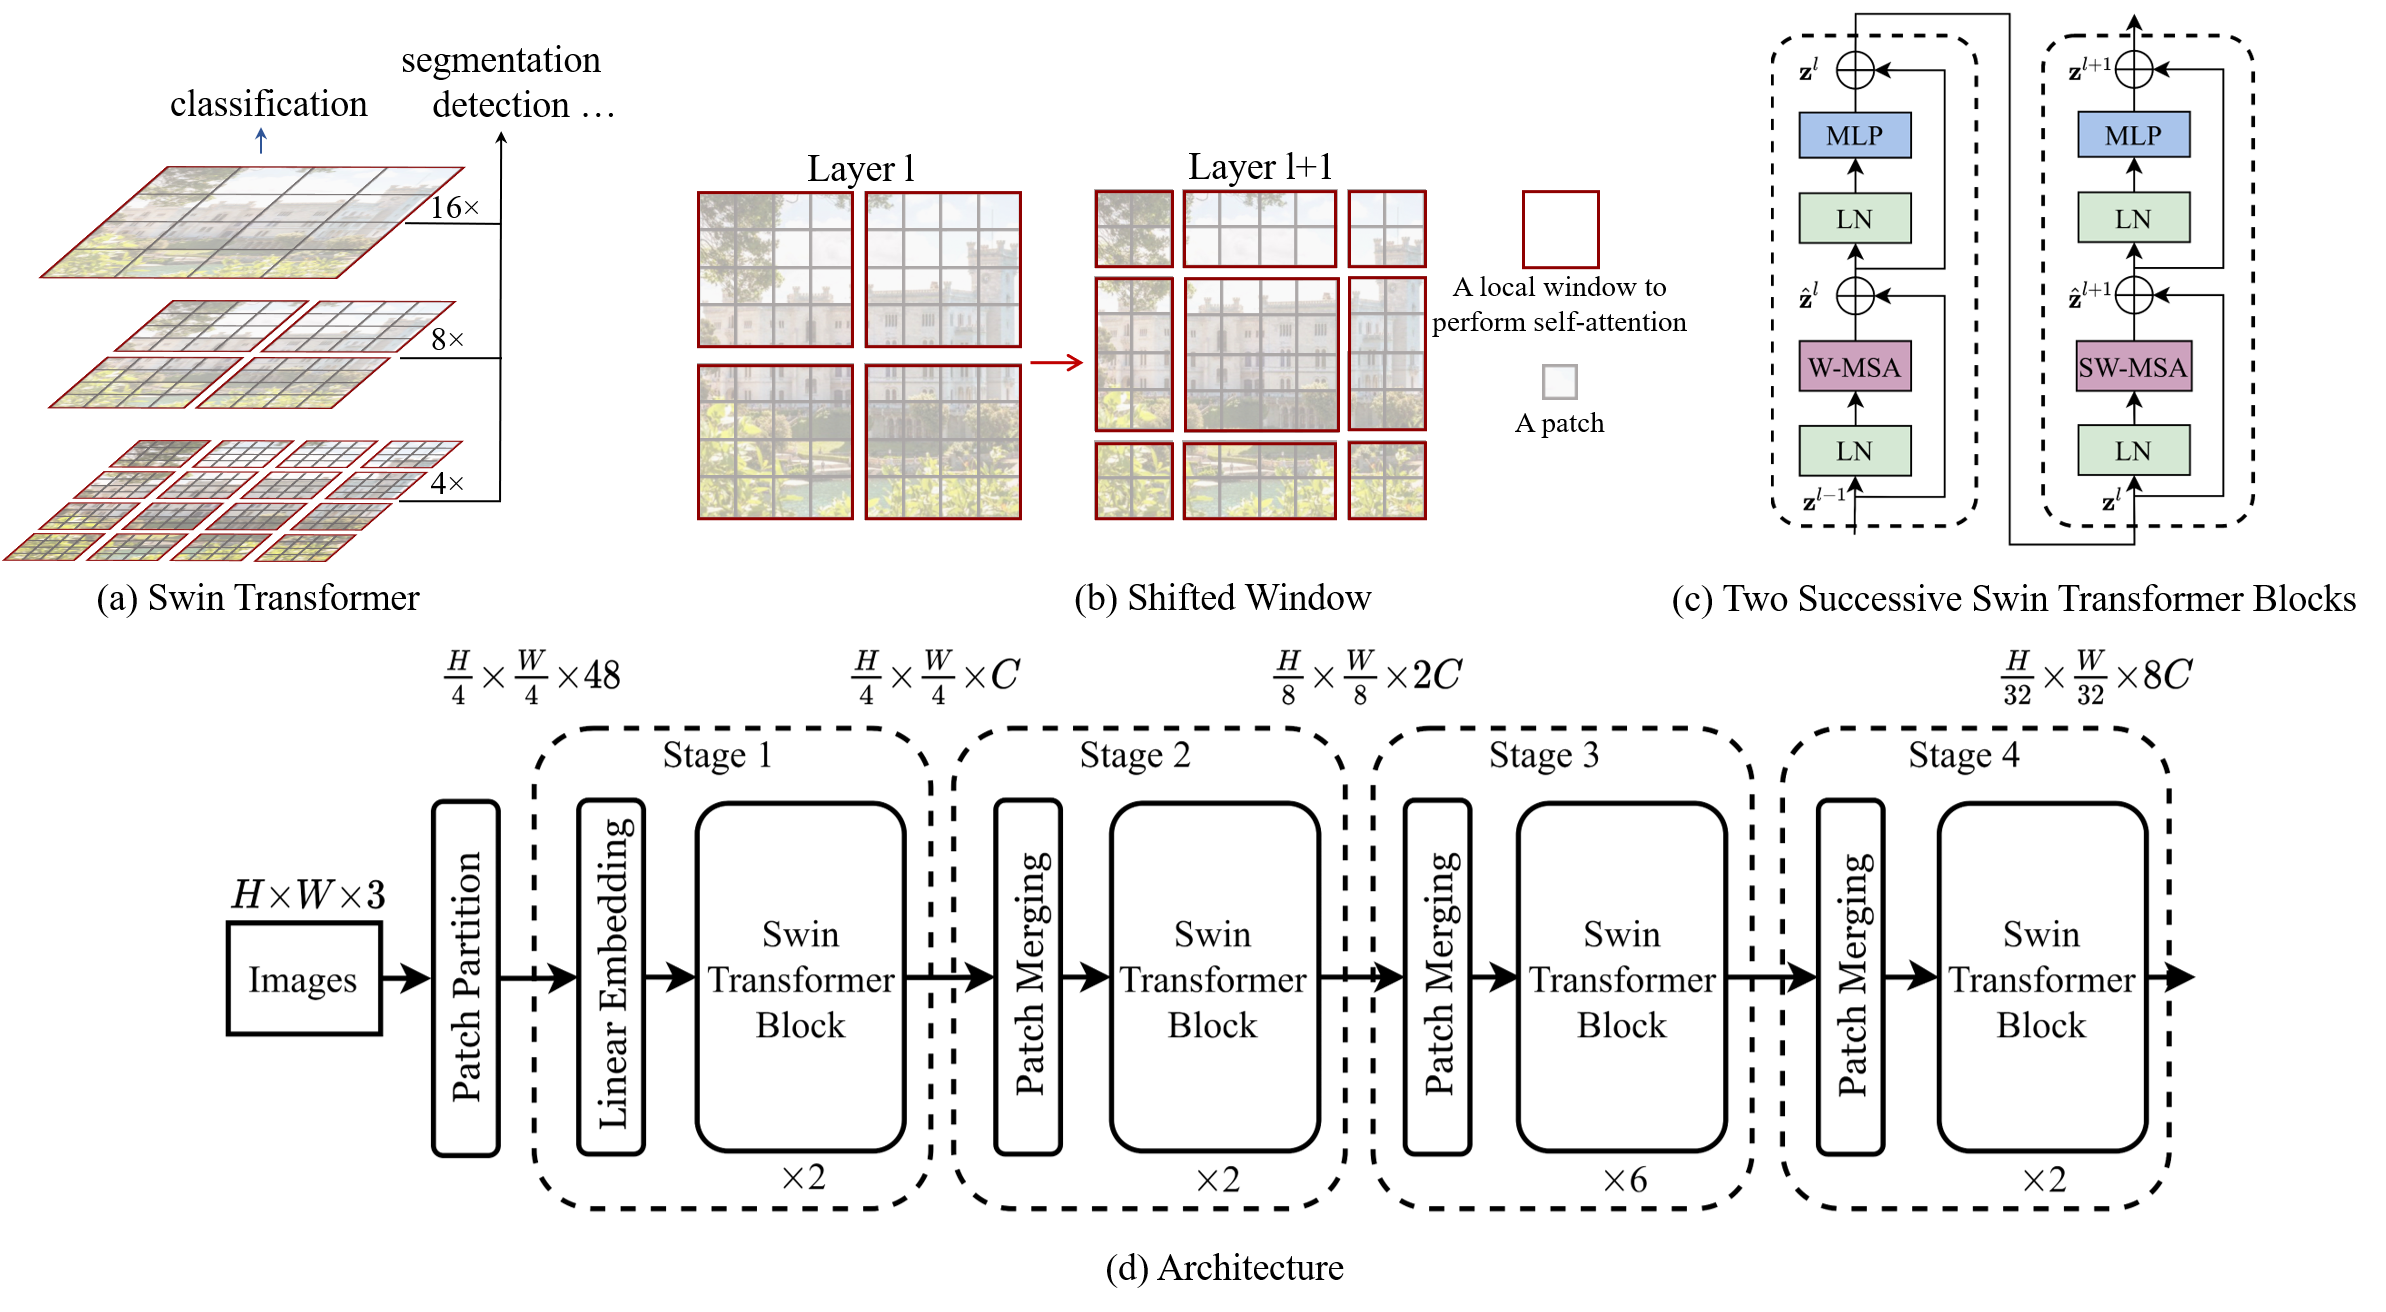
\includegraphics[width=\textwidth]{transformer_images/swin_transformer.png}
		\caption{مبدل پنجره متحرک}
		\label{fig: swin transformer}
	\end{minipage}
	\hfill
\end{figure}

در مبدل پنجره‌ای متحرک، به‌جای آن‌که مدل به تمام پچ‌ها در یک سطح ویژگی نگاه کند، تصویر را به «پنجره‌های محلی» \footnote{\lr{Local Windows}} تقسیم می‌کند و توجه را محدود به همان ناحیه می‌سازد \cite{liu2021swintransformer}. سپس با تکنیک جابه‌جایی \footnote{\lr{Shift}} این پنجره‌ها در لایه‌های بعدی، توان مدل برای ترکیب اطلاعات از نواحی مختلف تصویر (و در نهایت دیدن کل تصویر) افزایش پیدا می‌کند. این رویکرد، ایدهٔ کلیدی‌ای بود که باعث شد مدل هم محاسبات سبک‌تری داشته باشد و هم بتواند ارتباط‌های جهانی \footnote{\lr{Global}} را در طول لایه‌ها به‌دست آورد.



یکی دیگر از ایده‌های مهم در در مبدل پنجره‌ای متحرک، کوچک‌ کردن تدریجی نقشهٔ ویژگی  در طول معماری است؛ مشابه کاری که در \lr{ResNet} یا سایر \lr{CNN}ها انجام می‌شود \cite{he2016deep}. این امر ضمن کاهش هزینه محاسباتی، باعث می‌شود مدل بتواند با سطوح مختلفی از ویژگی‌ها کار کند و در نهایت خروجی نهایی باکیفیت‌تری ارائه دهد.

\subsection{قطعه‌بندی پچ در مبدل پنجره متحرک}
فرض کنیم تصویر ورودی \(\displaystyle I\) دارای ابعاد \(\displaystyle (H \times W \times 3)\) باشد. گام نخست، تقسیم تصویر به پچ‌های کوچک \(\displaystyle (P \times P)\) است \cite{dosovitskiy2020image}. اگر \(P\) اندازهٔ پچ \footnote{\lr{patch size}} باشد، آنگاه تعداد پچ‌ها در بعد افقی و عمودی، به‌ترتیب \(\displaystyle \frac{H}{P}\) و \(\displaystyle \frac{W}{P}\) خواهد بود. هر پچ را می‌توان به‌صورت یک بردار درآورد:

\[
X_{\text{patch}} \in \mathbb{R}^{(P^2 \cdot 3)}.
\]

سپس کل تصویر به \(\displaystyle \frac{H}{P} \times \frac{W}{P}\) پچ تبدیل خواهد شد و در نتیجه، ماتریس \(\displaystyle X\) از کنار هم قرار گرفتن این پچ‌ها به صورت زیر به‌دست می‌آید:

\[
X \in \mathbb{R}^{\Bigl(\frac{H}{P} \cdot \frac{W}{P}\Bigr) \times \Bigl(P^2 \cdot 3\Bigr)}.
\]

برخلاف مبدل بینایی اصلی این کاردر مبدل پنجره متحرک با استفاده از کانولوشن \footnote{\lr{convolution}} انجام می شود.
در واقع سایز کرنل در کانولوشن همان فضای برداری هر پچ هست که ما فرض میکنیم سایز کرنل برابر c ‌است. پس درنتیجه



\begin{equation}
	Z = X \cdot W_{\text{embed}} + b_{\text{embed}}, 
	\quad
	Z \in \mathbb{R}^{\Bigl(\tfrac{H}{P} \cdot \tfrac{W}{P}\Bigr) \times C}.
\end{equation}

در عمل، این عملیات معادل یک تبدیل خطی ساده است:

\[
W_{\text{embed}} \in \mathbb{R}^{\bigl(P^2 \cdot 3\bigr) \times C},
\quad
b_{\text{embed}} \in \mathbb{R}^{C}.
\]

پس از این مرحله، ما در هر موقعیت \((h, w)\) (از شبکهٔ پچ‌ها) یک بردار 
\(\displaystyle z_{h,w} \in \mathbb{R}^{C}\) داریم. این ماتریس \(\displaystyle Z\) 
ورودیِ اولین مرحله (\lr{Stage}) از مبدل های پنجره متحرک خواهد بود \cite{liu2021swintransformer}.

هر بلوک مبدل پنجره متحرک از چند بخش اصلی تشکیل شده است \cite{liu2021swintransformer}:

\begin{itemize}
	\item پنجره‌بندی تصویر \footnote{\lr{Window Partition}} 
	یا پنجره‌بندی جابه‌جاشده \footnote{\lr{Shifted Window Partition}}
	\item اعمال توجه چمد سر پنجره ای \footnote{\lr{Window Multi-Head Self Attention}}
	\item لایهٔ \lr{Skip Connection}\footnote{\lr{Skip Connection}} و \lr{Layer Norm}\footnote{\lr{Layer Norm}}
	\item مسیر پرسیپترون چندلایه \footnote{\lr{MLP}}:
% 	\begin{itemize}
% 			\item یک لایهٔ \lr{MLP} شامل دو لایهٔ \lr{Fully-Connected}\footnote{\lr{Fully-Connected}} 
	% 		و تابع فعال‌ساز \lr{GeLU}\footnote{\lr{GeLU}} % 	(یا تابع مشابه)
% 			\item لایهٔ \lr{Skip Connection}\footnote{\lr{Skip Connection}} و \lr{Layer Norm}\footnote{\lr{Layer Norm}}
% 	\end{itemize}
\end{itemize}




\subsection{توجه چند سر پنجره ای}

\subsubsection{تعریف پنجره‌های محلی}

در مبدل های پنجره متحرک، به‌جای آن‌که تمام پیکسل‌های یک نقشهٔ ویژگی بزرگ را یک‌جا 
در محاسبهٔ توجه  درگیر کنیم، نقشهٔ ویژگی را به قطعه‌های کوچکی به‌اندازه
\(\displaystyle (M \times M)\) تقسیم می‌کنیم. این قطعه‌های کوچک را 
«پنجره‌های محلی» می‌نامیم.

اگر اندازهٔ نقشهٔ ویژگی در یک لایه 
\(\displaystyle (H' \times W')\) باشد، 
با تقسیم آن به پنجره‌های 
\(\displaystyle (M \times M)\)، 
در راستای طول تقریباً 
\(\displaystyle \tfrac{H'}{M}\) پنجره خواهیم داشت 
و در راستای عرض هم 
\(\displaystyle \tfrac{W'}{M}\) پنجره.
(برای راحتی، فرض می‌کنیم 
\(\displaystyle H'\) و \(\displaystyle W'\) 
دقیقاً مضربی از \(\displaystyle M\) باشند 
تا تقسیم بدون باقی‌مانده انجام شود.)

هر کدام از این پنجره‌های 
\(\displaystyle (M \times M)\) 
دارای 
\(\displaystyle M^2\) پیکسل (یا موقعیت مکانی) است، 
و در هر پیکسل هم یک بردار ویژگی با بعد \(\displaystyle C\) قرار دارد.

به بیان ساده‌تر:
\begin{itemize}
	\item نقشهٔ ویژگی مثل یک صفحهٔ بزرگ است.
	\item آن را مانند شطرنج به مربع‌های کوچکی \(\displaystyle (M \times M)\) بخش می‌کنیم.
	\item در هر مربع (پنجره)، فقط به همان مربع نگاه می‌کنیم و محاسبات  توجه  را انجام می‌دهیم.
	\item این کار باعث می‌شود تعداد پیکسل‌هایی که درگیر محاسبهٔ توجه هستند، 
	به‌مراتب کمتر شود و هزینهٔ محاسباتی کاهش یابد.
\end{itemize}


\subsection{توجه}

برای هر بلوک، ابتدا بردارهای پرسش، کلید، مقدار ساخته می‌شوند. 
اگر \(\displaystyle z_i \in \mathbb{R}^C\) بردار ورودی مربوط به موقعیت \(i\) باشد، آنگاه:

\[
q_i = z_i W_Q, 
\quad
k_i = z_i W_K,
\quad
v_i = z_i W_V,
\]
که 
\[
W_Q, W_K, W_V \;\;\in \;\;\mathbb{R}^{C \times d}.
\]

پارامتر \(\displaystyle d\) معمولاً به‌صورت \(\displaystyle \tfrac{C}{h}\) در نظر گرفته می‌شود 
که در آن \(\displaystyle h\) تعداد سربندی  سر ها است. 
در توجه چند سر، خروجی نهایی با ترکیب \(\displaystyle h\) سر توجه محاسبه می‌شود.

در یک سر توجه، توجه به‌صورت زیر تعریف می‌شود:

\[
\mathrm{Attention}(Q, K, V)
=
\mathrm{Softmax}\Bigl(\frac{QK^\top}{\sqrt{d}}\Bigr)\,V,
\]

که در آن:

\begin{itemize}
	\item \(\displaystyle Q, K, V\) به‌ترتیب ماتریس‌هایی هستند که از کنار هم قرار دادن 
	\(\displaystyle q_i, k_i, v_i\) (برای تمام پیکسل‌های آن پنجره) ساخته می‌شوند.
	\item \(\displaystyle \sqrt{d}\): عامل مقیاس‌کننده برای جلوگیری از بزرگ شدن بیش‌ازحد ضرب داخلی است.
\end{itemize}

در مبدل های پنجره متحرک، این محاسبات به‌صورت پنجره‌ای انجام می‌شوند؛ یعنی 
برای هر پنجره، تنها پیکسل‌های داخل همان پنجره در ماتریس‌های 
\(\displaystyle Q\)، \(\displaystyle K\) و \(\displaystyle V\) لحاظ می‌شوند. 
به این ترتیب، زمان محاسبه و مصرف حافظه به‌شدت کاهش می‌یابد 
(در مقایسه با مبدل های بینایی که همه‌چیز را با هم مقایسه می‌کند).

تعداد سربندی \(\displaystyle h\) معمولاً طوری انتخاب می‌شود که 
\(\displaystyle C = h \times d.\) 
خروجی هر سر پس از محاسبه توجه به‌صورت زیر با هم ادغام می‌شوند:

\[
\mathrm{MultiHead}(Q,K,V) 
= 
\bigl[\text{head}_1,\ \text{head}_2,\ \dots,\ \text{head}_h\bigr]\,
W_O,
\]
که 
\[
\text{head}_j = \mathrm{Attention}\bigl(Q_j,\ K_j,\ V_j\bigr),
\quad 
W_O \in \mathbb{R}^{C \times C}
\]
ماتریس ترکیب نهایی است.

\subsection{پنجره متحرک جا به جا شده}

در مدبل های پنجر متحرک، ایدهٔ «پنجره‌های جابه‌جاشده»    \footnote{\lr{Shifted Windows}}
به این منظور ارائه شده است تا مدل، ارتباط پیکسل‌های واقع در پنجره‌های مجاور را هم یاد بگیرد \cite{liu2021swintransformer}.
اگر فقط از پنجره‌های ثابت (بدون جابه‌جایی) استفاده کنیم، هر بلوک از تصویر تنها با پیکسل‌های همان 
پنجره در ارتباط خواهد بود و ممکن است اطلاعات نواحی مرزی با نواحی مجاور به‌خوبی تبادل نشود.

روش مبدل های پنجره متحرک برای رفع این محدودیت از یک تکنیک ساده اما مؤثر استفاده می‌کند \cite{liu2021swintransformer}:
\begin{itemize}
	\item در یک لایه، محاسبات توجه در پنجره‌های محلی ثابت انجام می‌شود.
	\item در لایهٔ بعدی، پنجره‌ها به اندازه‌ای مشخص جابه‌جا می‌شوند (به‌صورت شیفت افقی و عمودی) 
	تا نواحی مرزی نیز در محاسبات گنجانده شوند.
	\item این فرآیند باعث می‌شود که پیکسل‌ها در پنجره‌های مختلف (و در مرزهای مختلف) 
	در محاسبات دخیل شوند و تبادل اطلاعات بهتری میان نواحی تصویر رخ دهد.
\end{itemize}

\subsubsection{توجه چند سری پنجره ای}
در توجه چندسری پنجره ای \footnote{\lr{W-MSA}}، نقشهٔ ویژگی به پنجره‌های \(\displaystyle (M \times M)\) تقسیم می‌شود \cite{liu2021swintransformer}.
هیچ جابه‌جایی در این تقسیم‌بندی وجود ندارد؛ یعنی اگر نقشهٔ ویژگی را یک مستطیل بزرگ در نظر بگیریم،
آن را شبیه کاشی‌کاری یا شطرنج‌بندی به بلوک‌های مربعی \(\displaystyle (M \times M)\) برش می‌زنیم.
در این حالت، پیکسل‌های هر پنجره فقط با همدیگر (درون همان پنجره) ارتباط برقرار می‌کنند.

\subsubsection{توجه چند سری پنجره ای جا به جا شده}
مطابق شکل \ref{fig:Cycle Shift in Swin Tranformer}، بعد از اینکه بلوک اول (توجه چند سری پنجره ای) کارش تمام شد، در بلوک دوم، قبل از تقسیم‌بندی به پنجره‌های 
\(\displaystyle (M \times M)\)، نقشهٔ ویژگی را جابه‌جا  می‌کنیم \cite{liu2021swintransformer}.
در مقالهٔ اصلی، این مقدار جابه‌جایی معمولاً نیمِ اندازهٔ پنجره 
\(\displaystyle \frac{M}{2}\)
در راستای افقی و عمودی است. به این ترتیب:

\begin{itemize}
	\item پیکسل‌هایی که پیش از این در دو پنجرهٔ جداگانه قرار داشتند، ممکن است حالا به دلیل جابه‌جایی وارد یک پنجرهٔ مشترک شوند.
	\item مدل حالا می‌تواند بین این پیکسل‌های «مرزی» نیز  توجه برقرار کند و اطلاعات را بهتر مبادله کند.
\end{itemize}

با این جابه‌جایی، بخشی از پیکسل‌ها در نقشهٔ ویژگی از یک طرف «خارج» می‌شوند. برای اینکه این پیکسل‌ها را از دست ندهیم، از ترفندی به نام  جابجایی چرخه‌ای \footnote{\lr{Cyclic Shift}} استفاده می‌شود. در جا به جایی چرخه ای ، پیکسل‌هایی که از سمت راست بیرون می‌روند دوباره از سمت چپ وارد می‌شوند و بالعکس؛ درست شبیه وقتی که یک تصویر را به‌صورت حلقه‌ای اسکرول می‌کنیم \footnote{\lr{Wrap around}}. مثالی از جا به جایی چرخه ای  در شکل \ref{fig:Cycle Shift in Swin Tranformer} آمده است.

\begin{figure}[h]
	\centering
	\begin{minipage}[b]{1\textwidth}
		\centering
		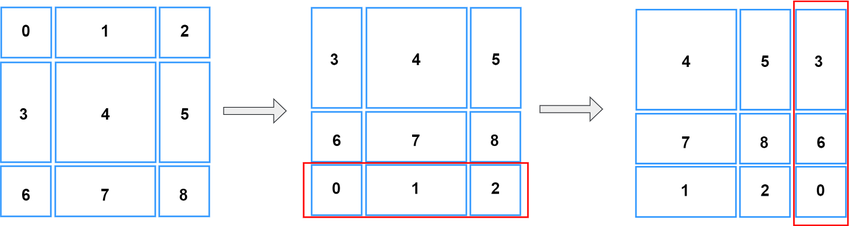
\includegraphics[width=\textwidth]{transformer_images/cycle_shift.png}
		\caption{جا به جایی چرخه ای}
		\label{fig:Cycle Shift in Swin Tranformer}
	\end{minipage}
	\hfill
\end{figure}

در بلوک اول (بدون جابه‌جایی)، پنجره‌ها ثابت‌اند و پیکسل‌های مرزی در هر پنجره ممکن است فرصت کافی برای تبادل اطلاعات با پیکسل‌های مرزیِ پنجرهٔ کناری را نداشته باشند.

در بلوک دوم (جابه‌جاشده)، مرزهای پنجره‌ها تغییر می‌کند و برخی پیکسل‌هایی که قبلاً در پنجره‌های جدا بودند، اکنون در یک پنجرهٔ مشترک‌اند؛ در نتیجه مدل می‌تواند رابطه و همبستگی بین آن‌ها را هم یاد بگیرد.

این جابه‌جایی و قرارگیری مجدد پیکسل‌ها کنار هم در نهایت کمک می‌کند تا مدل بتواند اطلاعات کل تصویر را با هزینهٔ محاسباتی کمتر (نسبت به توجهِ سراسریِ کامل) در اختیار داشته باشد \cite{liu2021swintransformer}.

اگر بخواهیم با مثال توضیح دهیم، فرض کنید در یک تابلوی شطرنجی، خانه‌های کناری همدیگر را «نمی‌بینند» چون در دو بلوک مختلف هستند.
اما اگر کمی تابلوی شطرنجی را به سمت بالا-چپ یا پایین-راست جابه‌جا کنیم،
حالا بخشی از آن خانه‌ها وارد یک بلوک واحد می‌شوند و اطلاعاتشان با هم ترکیب می‌شود.
سپس به‌طور دوره‌ای (\textit{\lr{Cyclic}})، گوشه‌های اضافی را به آن سمت دیگر تابلوی شطرنجی می‌آوریم
تا هیچ چیز از دست نرود.

به این شکل، سِری اول و دوم بلوک‌های مبدل های پنجره متحرک 
تکمیل‌کنندهٔ یکدیگر می‌شوند \cite{liu2021swintransformer}:
\begin{itemize}
	\item \textbf{بلوک اول:} محاسبهٔ توجه در چهارچوب پنجره‌های ثابت.
	\item \textbf{بلوک دوم:} محاسبهٔ  توجه در پنجره‌های جابه‌جاشده که منجر به تعامل بیشتر بین مرزهای مختلف می‌شود.
\end{itemize}


\subsection{پرسپتروون چند لایه}
پس از انجام توجه چند سری پنجره ای جا  به جا شده 
خروجی به یک مسیر \textbf{\lr{MLP}} می‌رود \cite{liu2021swintransformer}. ساختار این \lr{MLP} به‌صورت زیر است:

\begin{equation}
	X' = \mathrm{GELU}(X W_1 + b_1) \; W_2 + b_2,
	\label{eq:gelu_transform}
\end{equation}

که در آن
\[
W_1 \in \mathbb{R}^{C \times (rC)}, 
\quad
W_2 \in \mathbb{R}^{(rC) \times C}
\]
هستند و \(\displaystyle r\) معمولاً ضریب افزایش بعد را نشان می‌دهد (مثلاً ۴). 

تابع فعال‌ساز \lr{GELU} (یا \lr{ReLU} و سایر توابع) نیز در این‌جا قابل استفاده است \cite{hendrycks2016gelu}.

\subsection{ترکیب پچ ها}
در مدل مبدل های پنجره متحرک، ساختار سلسله‌مراتبی به این معناست که ما در چند مرحله (\lr{Stage}) مختلف، نقشهٔ ویژگی را کوچک‌تر می‌کنیم و در عین حال، عمق (تعداد کانال‌های ویژگی) را افزایش می‌دهیم. هدف اصلی از این کار عبارت است از:

\begin{itemize}
	\item \textbf{استخراج ویژگی‌های سطح بالاتر:}
	وقتی نقشهٔ ویژگی کوچک‌تر می‌شود، هر واحد از نقشهٔ ویژگی بیانگر بخش گسترده‌تری از تصویر اصلی است؛ 
	پس مدل به‌تدریج جزئیات محلی را با درک کلی‌تری از تصویر جایگزین می‌کند \cite{he2016deep}.
	
	\item \textbf{کاهش هزینهٔ محاسبات:}
	در مراحل بعدی، چون ابعاد فضایی کمتر می‌شود، مدل راحت‌تر می‌تواند با ویژگی‌های جدید کار کند 
	(چون مثلاً به‌جای \((H \times W)\) پیکسل، تعداد کمتری پیکسل داریم) \cite{liu2021swintransformer}.
\end{itemize}


پس از چندین بلوک پردازشی، نقشهٔ ویژگی، ابعادی به شکل \((\tfrac{H}{P}, \tfrac{W}{P})\) با تعداد کانال \(\displaystyle C\) دارد. 
این یعنی پس از برش‌دادن تصویر به پچ‌ها و گذر از چند لایه، اکنون یک نقشهٔ ویژگی داریم که کوچک‌تر از تصویر اصلی است، 
اما هنوز ممکن است خیلی بزرگ باشد.

در مرحلهٔ بعد (\lr{Stage} بعدی)، می‌خواهیم این نقشه را نصف کنیم 
(یعنی طول و عرض را دو برابر کوچک کنیم) و در عوض عمق کانال را دو برابر کنیم 
(تا ظرفیت مدل در استخراج ویژگی‌های پیچیده‌تر بیشتر شود). برای انجام این کار از فرایندی به نام 
ترکیب پچ‌ها استفاده می‌کنیم.
\cite{liu2021swintransformer}:

\subsubsection{1. انتخاب بلوک‌های \((2 \times 2)\)}
ابتدا نقشهٔ ویژگی را در بُعد مکانی به بلوک‌های \((2 \times 2)\) تقسیم می‌کنیم.  
اگر \(\displaystyle Z_{i,j}\) ویژگیِ مکان \((i, j)\) باشد، 
یک بلوک \((2 \times 2)\) شامل چهار پیکسل است:
\[
Z_{2i, 2j}, \quad Z_{2i, 2j+1}, \quad Z_{2i+1, 2j}, \quad Z_{2i+1, 2j+1}.
\]

\subsubsection{2. ادغام ویژگی‌های چهار پیکسل}
برای هر بلوک \((2 \times 2)\)، این چهار پیکسل را در بُعد کانال به هم می‌چسبانیم.  
اگر هر پیکسل یک بردار از بعد \(\displaystyle C\) باشد، اکنون بعدِ حاصل از کنار هم گذاشتن این چهار پیکسل می‌شود \(\displaystyle 4C\).  
نام این بردار ادغام‌شده را \(\displaystyle Z'\) می‌گذاریم.

\subsubsection{3. لایهٔ خطی برای تغییر بعد}
وقتی چهار بردار \(\displaystyle C\)-بعدی را کنار هم می‌گذاریم، یک بردار \(\displaystyle 4C\)-بعدی شکل می‌گیرد.  
حال با یک لایهٔ خطی، بعدِ \(\displaystyle 4C\) را به بعد جدیدی تبدیل می‌کنیم.  
معمولاً این بعد جدید برابر \(\displaystyle 2C\) در نظر گرفته می‌شود؛ 
یعنی دو برابر بزرگ‌تر از قبل اما نه چهار برابر:
\begin{equation}
	Z' \mapsto Z'' = Z' \, W_{\text{merge}} + b_{\text{merge}},
	\label{eq:merge_transform}
\end{equation}

که بعد ویژگی را از \(\displaystyle 4C\) به \(\displaystyle 2C\) کاهش می‌دهد.

\subsubsection{4. کاهش ابعاد مکانی}
در عین حال، وقتی هر چهار پیکسل \((2 \times 2)\) را ادغام می‌کنیم، 
نقشهٔ ویژگی ما ابعاد فضایی \(\bigl(\tfrac{H}{2P} \times \tfrac{W}{2P}\bigr)\) خواهد داشت 
(چون هر بلوک \((2 \times 2)\) تبدیل به یک بردار می‌شود).

به عبارت دیگر، تعداد نقاط مکانی نصف می‌شود (هم در طول و هم در عرض)، 
اما کانال از \(\displaystyle C\) به \(\displaystyle 2C\) افزایش می‌یابد.

\begin{figure}[h]
	\centering
	\begin{minipage}[b]{1\textwidth}
		\centering
		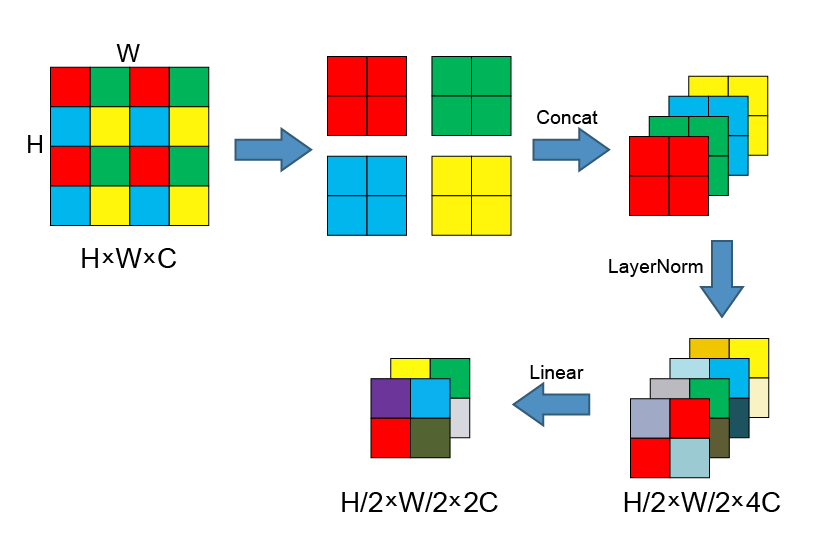
\includegraphics[width=\textwidth]{transformer_images/Patch_merging_new.png}
		\caption{ادغام پچ ها}
		\label{fig:patch merging in Swin Transformer}
	\end{minipage}
	\hfill
\end{figure}

در شبکه‌های کانولوشنی، مرتبا از لایه‌های ادغام \footnote{\lr{Pooling}} یا کانولوشن با گام \footnote{\lr{Stride-Convolution}} 
برای کوچک‌کردن ابعاد استفاده می‌شود تا اطلاعات سطح بالاتر (مثل ساختار کلی اشیا) راحت‌تر استخراج شود \cite{he2016deep}.  در مبدل پنجره متحرک هم همین ایدهٔ سلسله‌مراتب را به دنیای مبدل ها آورده است \cite{liu2021swintransformer}.  
همچنین اگر ابعاد فضایی را کم نکنیم، هزینهٔ توجه به‌شدت زیاد می‌شود 
(چون باید در هر لایه برای همهٔ پیکسل‌ها توجه محاسبه گردد).

در معماری کلی کبدل های پنجره متحرک، پس از \lr{Stage 1} و عبور از بلوک‌های توجه چند سر پنجره ای و توجه چند سر پنجره ای جابه جا شده، عملیات  ادغام پچ ها انجام می‌شود. سپس در \lr{Stage 2}، ویژگی‌های کوچک‌تری داریم، اما تعداد کانال‌ها افزایش یافته است \cite{liu2021swintransformer}.  
مشابه معماری‌های کانولوشنی، با افزایش عمق \footnote{\lr{Depth}}، ابعاد فضایی کاهش و تعداد کانال‌ها افزایش پیدا می‌کند.

در انتهای \lr{Stage} آخر، خروجی به یک لایهٔ \lr{FC} داده می‌شود تا تعداد کلاس‌ها را پیش‌بینی کند.  
پس از گذر از \lr{Softmax}، احتمال هر کلاس به‌دست می‌آید و مدل در نهایت کلاس نهایی را برمی‌گزیند.






